\PassOptionsToPackage{unicode=true}{hyperref} % options for packages loaded elsewhere
\PassOptionsToPackage{hyphens}{url}
%
\documentclass[]{book}
\usepackage{lmodern}
\usepackage{amssymb,amsmath}
\usepackage{ifxetex,ifluatex}
\usepackage{fixltx2e} % provides \textsubscript
\ifnum 0\ifxetex 1\fi\ifluatex 1\fi=0 % if pdftex
  \usepackage[T1]{fontenc}
  \usepackage[utf8]{inputenc}
  \usepackage{textcomp} % provides euro and other symbols
\else % if luatex or xelatex
  \usepackage{unicode-math}
  \defaultfontfeatures{Ligatures=TeX,Scale=MatchLowercase}
\fi
% use upquote if available, for straight quotes in verbatim environments
\IfFileExists{upquote.sty}{\usepackage{upquote}}{}
% use microtype if available
\IfFileExists{microtype.sty}{%
\usepackage[]{microtype}
\UseMicrotypeSet[protrusion]{basicmath} % disable protrusion for tt fonts
}{}
\IfFileExists{parskip.sty}{%
\usepackage{parskip}
}{% else
\setlength{\parindent}{0pt}
\setlength{\parskip}{6pt plus 2pt minus 1pt}
}
\usepackage{hyperref}
\hypersetup{
            pdftitle={Outstanding User Interfaces with Shiny},
            pdfauthor={David Granjon},
            pdfborder={0 0 0},
            breaklinks=true}
\urlstyle{same}  % don't use monospace font for urls
\usepackage{color}
\usepackage{fancyvrb}
\newcommand{\VerbBar}{|}
\newcommand{\VERB}{\Verb[commandchars=\\\{\}]}
\DefineVerbatimEnvironment{Highlighting}{Verbatim}{commandchars=\\\{\}}
% Add ',fontsize=\small' for more characters per line
\usepackage{framed}
\definecolor{shadecolor}{RGB}{248,248,248}
\newenvironment{Shaded}{\begin{snugshade}}{\end{snugshade}}
\newcommand{\AlertTok}[1]{\textcolor[rgb]{0.94,0.16,0.16}{#1}}
\newcommand{\AnnotationTok}[1]{\textcolor[rgb]{0.56,0.35,0.01}{\textbf{\textit{#1}}}}
\newcommand{\AttributeTok}[1]{\textcolor[rgb]{0.77,0.63,0.00}{#1}}
\newcommand{\BaseNTok}[1]{\textcolor[rgb]{0.00,0.00,0.81}{#1}}
\newcommand{\BuiltInTok}[1]{#1}
\newcommand{\CharTok}[1]{\textcolor[rgb]{0.31,0.60,0.02}{#1}}
\newcommand{\CommentTok}[1]{\textcolor[rgb]{0.56,0.35,0.01}{\textit{#1}}}
\newcommand{\CommentVarTok}[1]{\textcolor[rgb]{0.56,0.35,0.01}{\textbf{\textit{#1}}}}
\newcommand{\ConstantTok}[1]{\textcolor[rgb]{0.00,0.00,0.00}{#1}}
\newcommand{\ControlFlowTok}[1]{\textcolor[rgb]{0.13,0.29,0.53}{\textbf{#1}}}
\newcommand{\DataTypeTok}[1]{\textcolor[rgb]{0.13,0.29,0.53}{#1}}
\newcommand{\DecValTok}[1]{\textcolor[rgb]{0.00,0.00,0.81}{#1}}
\newcommand{\DocumentationTok}[1]{\textcolor[rgb]{0.56,0.35,0.01}{\textbf{\textit{#1}}}}
\newcommand{\ErrorTok}[1]{\textcolor[rgb]{0.64,0.00,0.00}{\textbf{#1}}}
\newcommand{\ExtensionTok}[1]{#1}
\newcommand{\FloatTok}[1]{\textcolor[rgb]{0.00,0.00,0.81}{#1}}
\newcommand{\FunctionTok}[1]{\textcolor[rgb]{0.00,0.00,0.00}{#1}}
\newcommand{\ImportTok}[1]{#1}
\newcommand{\InformationTok}[1]{\textcolor[rgb]{0.56,0.35,0.01}{\textbf{\textit{#1}}}}
\newcommand{\KeywordTok}[1]{\textcolor[rgb]{0.13,0.29,0.53}{\textbf{#1}}}
\newcommand{\NormalTok}[1]{#1}
\newcommand{\OperatorTok}[1]{\textcolor[rgb]{0.81,0.36,0.00}{\textbf{#1}}}
\newcommand{\OtherTok}[1]{\textcolor[rgb]{0.56,0.35,0.01}{#1}}
\newcommand{\PreprocessorTok}[1]{\textcolor[rgb]{0.56,0.35,0.01}{\textit{#1}}}
\newcommand{\RegionMarkerTok}[1]{#1}
\newcommand{\SpecialCharTok}[1]{\textcolor[rgb]{0.00,0.00,0.00}{#1}}
\newcommand{\SpecialStringTok}[1]{\textcolor[rgb]{0.31,0.60,0.02}{#1}}
\newcommand{\StringTok}[1]{\textcolor[rgb]{0.31,0.60,0.02}{#1}}
\newcommand{\VariableTok}[1]{\textcolor[rgb]{0.00,0.00,0.00}{#1}}
\newcommand{\VerbatimStringTok}[1]{\textcolor[rgb]{0.31,0.60,0.02}{#1}}
\newcommand{\WarningTok}[1]{\textcolor[rgb]{0.56,0.35,0.01}{\textbf{\textit{#1}}}}
\usepackage{longtable,booktabs}
% Fix footnotes in tables (requires footnote package)
\IfFileExists{footnote.sty}{\usepackage{footnote}\makesavenoteenv{longtable}}{}
\usepackage{graphicx,grffile}
\makeatletter
\def\maxwidth{\ifdim\Gin@nat@width>\linewidth\linewidth\else\Gin@nat@width\fi}
\def\maxheight{\ifdim\Gin@nat@height>\textheight\textheight\else\Gin@nat@height\fi}
\makeatother
% Scale images if necessary, so that they will not overflow the page
% margins by default, and it is still possible to overwrite the defaults
% using explicit options in \includegraphics[width, height, ...]{}
\setkeys{Gin}{width=\maxwidth,height=\maxheight,keepaspectratio}
\setlength{\emergencystretch}{3em}  % prevent overfull lines
\providecommand{\tightlist}{%
  \setlength{\itemsep}{0pt}\setlength{\parskip}{0pt}}
\setcounter{secnumdepth}{5}
% Redefines (sub)paragraphs to behave more like sections
\ifx\paragraph\undefined\else
\let\oldparagraph\paragraph
\renewcommand{\paragraph}[1]{\oldparagraph{#1}\mbox{}}
\fi
\ifx\subparagraph\undefined\else
\let\oldsubparagraph\subparagraph
\renewcommand{\subparagraph}[1]{\oldsubparagraph{#1}\mbox{}}
\fi

% set default figure placement to htbp
\makeatletter
\def\fps@figure{htbp}
\makeatother

\usepackage{booktabs}
\usepackage{amsthm}
\makeatletter
\def\thm@space@setup{%
  \thm@preskip=8pt plus 2pt minus 4pt
  \thm@postskip=\thm@preskip
}
\makeatother
\usepackage[]{natbib}
\bibliographystyle{apalike}

\title{Outstanding User Interfaces with Shiny}
\author{David Granjon}
\date{2020-05-09}

\begin{document}
\maketitle

{
\setcounter{tocdepth}{1}
\tableofcontents
}
\hypertarget{prerequisites}{%
\chapter*{Prerequisites}\label{prerequisites}}
\addcontentsline{toc}{chapter}{Prerequisites}

\begin{itemize}
\tightlist
\item
  Be familiar with \href{https://mastering-shiny.org}{Shiny}
\item
  Basic knowledge in HTML and JavaScript is a plus but not mandatory
\end{itemize}

\hypertarget{disclaimer}{%
\section*{Disclaimer}\label{disclaimer}}
\addcontentsline{toc}{section}{Disclaimer}

This book is not an HTML/Javascript/CSS course! Instead, it provides a \emph{survival kit} to be able to customize Shiny. I am sure however that readers will want to explore more about these topics.

\hypertarget{is-this-book-for-me}{%
\section*{Is this book for me?}\label{is-this-book-for-me}}
\addcontentsline{toc}{section}{Is this book for me?}

You should read this book if you answer yes to the following questions:

\begin{itemize}
\tightlist
\item
  Do you want to know how to develop outstanding shiny apps?
\item
  Have you ever wondered how to develop new input widgets?
\end{itemize}

\hypertarget{related-content}{%
\section*{Related content}\label{related-content}}
\addcontentsline{toc}{section}{Related content}

See the \href{https://rstudio.cloud}{RStudio Cloud} dedicated project.

\begin{Shaded}
\begin{Highlighting}[]
\KeywordTok{library}\NormalTok{(shiny)}
\KeywordTok{library}\NormalTok{(shinydashboard)}
\KeywordTok{library}\NormalTok{(shiny.semantic)}
\KeywordTok{library}\NormalTok{(cascadess)}
\KeywordTok{library}\NormalTok{(htmltools)}
\KeywordTok{library}\NormalTok{(purrr)}
\KeywordTok{library}\NormalTok{(magrittr)}
\end{Highlighting}
\end{Shaded}

\hypertarget{intro}{%
\chapter{Introduction}\label{intro}}

There are various Shiny focused resources introducing basic as well as advanced topics such as modules and Javascript/R interactions. However, handling advanced user interfaces was never an emphasis. Clients often desire custom designs, yet this generally exceeds core features of Shiny. We recognized that R App developers lacking a significant background in web development may have found this requirement to be overwhelming. Consequently, the aim of this book is to provide readers the necessary knowledge to extend Shiny's layout, input widgets and output elements. This book is organized into four parts. We first go through the basics of HTML, JavaScript and jQuery. In part 2, we dive into the \{htmltools\} package, providing functions to create and manipulate shiny tags as well as manage dependencies. Part 3 homes in on the development of a new template on top of Shiny by demonstrating examples from the \{bs4Dash\} and \{shinyMobile\} packages, part of the RinteRface project.

\hypertarget{part-survival-kit}{%
\part*{Survival Kit}\label{part-survival-kit}}
\addcontentsline{toc}{part}{Survival Kit}

This part will give you basis in HTML, JavaScript to get started\ldots{}

\hypertarget{survival-kit-html}{%
\chapter{HTML}\label{survival-kit-html}}

In the following, we will give a short introduction to the HTML language. First of all, let's do the following experience:

\begin{itemize}
\tightlist
\item
  Open your RStudio IDE
\item
  Load shiny with \texttt{library(shiny)}
\item
  Execute \texttt{p("Hello\ World")} and notice the output format
\item
  This is an HTML tag!
\end{itemize}

\hypertarget{html-basics}{%
\section{HTML Basics}\label{html-basics}}

HTML (Hypertext Markup Language) is derived from the SGML (Standard Generalized markup Language). An HTML file contains tags that can be divided into 2 catagories:

\begin{itemize}
\tightlist
\item
  paired-tags
\item
  closing-tags
\end{itemize}

\begin{Shaded}
\begin{Highlighting}[]
\CommentTok{<!-- /* paired-tags */ -->}
\KeywordTok{<p></p>}
\KeywordTok{<div></div>}

\CommentTok{<!-- /* self-closing tags */ -->}
\KeywordTok{<iframe/>}
\KeywordTok{<img/>}
\KeywordTok{<input/>}
\KeywordTok{<br/>}
\end{Highlighting}
\end{Shaded}

\hypertarget{tag-attributes}{%
\section{Tag attributes}\label{tag-attributes}}

All tags above don't have any attributes. Yet HTML allows to set attributes inside each tag. There exist a large range of attributes and we will only see 2 of them for now:

\begin{itemize}
\tightlist
\item
  class: may be shared between multiple tags
\item
  id: each must be unique
\end{itemize}

\begin{Shaded}
\begin{Highlighting}[]
\KeywordTok{<div}\OtherTok{ class=}\StringTok{"awesome-item"}\OtherTok{ id=}\StringTok{"myitem"}\KeywordTok{></div>}
\CommentTok{<!-- /* the class awesome-item may be applied to multiple tags */ -->}
\KeywordTok{<span}\OtherTok{ class=}\StringTok{"awesome-item"}\KeywordTok{></span>}
\end{Highlighting}
\end{Shaded}

Both attributes are widely used by CSS and JavaScript (we will discover in the following chapter the jQuery selectors) to apply custom style to a web page. While class may apply to multiple elements, id is restricted to only one item.

\hypertarget{html-page-skeleton}{%
\section{HTML page: skeleton}\label{html-page-skeleton}}

An HTML page is a collection of tags which will be interpreted by the web browser step by step. The simplest HTML page may be defined as follows:

\begin{Shaded}
\begin{Highlighting}[]
\DataTypeTok{<!DOCTYPE }\NormalTok{HTML}\DataTypeTok{>}
\KeywordTok{<html>}
  \KeywordTok{<head>}
  \CommentTok{<!-- /* head content here */ -->}
  \KeywordTok{</head>}
  \KeywordTok{<body>}
  \CommentTok{<!-- /* body content here */ -->}
  \KeywordTok{</body>}
\KeywordTok{</html>}
\end{Highlighting}
\end{Shaded}

\begin{itemize}
\tightlist
\item
  \texttt{\textless{}html\textgreater{}} is the may wrapper
\item
  \texttt{\textless{}head\textgreater{}} and \texttt{\textless{}body\textgreater{}} are the 2 main children
\end{itemize}

\texttt{\textless{}head\textgreater{}} contains dependencies like styles and JavaScript files (but not only), \texttt{\textless{}body\textgreater{}} contains the page content. We will see later that JavaScript files are often added just before the end of the \texttt{\textless{}body\textgreater{}}.

Only the body content is displayed on the screen!

Let's write the famous Hello World in html:

\begin{Shaded}
\begin{Highlighting}[]
\DataTypeTok{<!DOCTYPE }\NormalTok{HTML}\DataTypeTok{>}
\KeywordTok{<html>}
  \KeywordTok{<head>}
  \CommentTok{<!-- head content here -->}
  \KeywordTok{</head>}
  \KeywordTok{<body>}
  \KeywordTok{<p>}\NormalTok{Hello World}\KeywordTok{</p>}
  \KeywordTok{</body>}
\KeywordTok{</html>}
\end{Highlighting}
\end{Shaded}

In order to preview this page in a web browser, you need to save the above snippet to a script \texttt{hello-world.html} and double-click on it. It will open with you default web browser.

\hypertarget{about-the-dom}{%
\section{About the DOM}\label{about-the-dom}}

The DOM stands for ``Document Object Model'', is a convenient representation of the html document. There actually exists multiple DOM types, namely DOM-XML and DOM-HTML but we will only focus on the later (in the following DOM is DOM-HTML).
If we consider the last example (Hello World), the associated DOM tree may be inspected in Figure \ref{fig:html-dom}.

\hypertarget{visualizing-the-dom-the-html-inspector}{%
\subsection{Visualizing the DOM: the HTML inspector}\label{visualizing-the-dom-the-html-inspector}}

Below, we introduce a tool that we is going to be a valuable ally during our ambitious quest to beautiful shiny user interfaces. In this chapter, we restrict the description to the first panel of the HTML inspector \footnote{As shown in Figure \ref{fig:html-dom}, the inspector also has tools to debug JavaScript code, inspect files, run performances audit, \ldots{} We will describe some of these later in the book.}. This feature is available in all web browser but we will only focus on Chrome.

\begin{itemize}
\tightlist
\item
  Open the hello-world.html example in a web browser (google chrome here)
\item
  Right-click to open the HTML inspector (developer tools must be enabled if it is not the case)
\end{itemize}

The HTML inspector in a convenient tool to explore the structure of the current HTML page. On the left-hand side, the DOM tree is displayed and we clearly see that \texttt{\textless{}html\textgreater{}} is the parent of \texttt{\textless{}head\textgreater{}} and \texttt{\textless{}body\textgreater{}}. \texttt{\textless{}body\textgreater{}} has also 1 child, that is \texttt{\textless{}p\textgreater{}}. We didn't mention this yet but we can preview any style (CSS) associated to the selected element on the right panel as well as Event Listeners (JavaScript). We will discuss that in the next chapter.

\begin{figure}
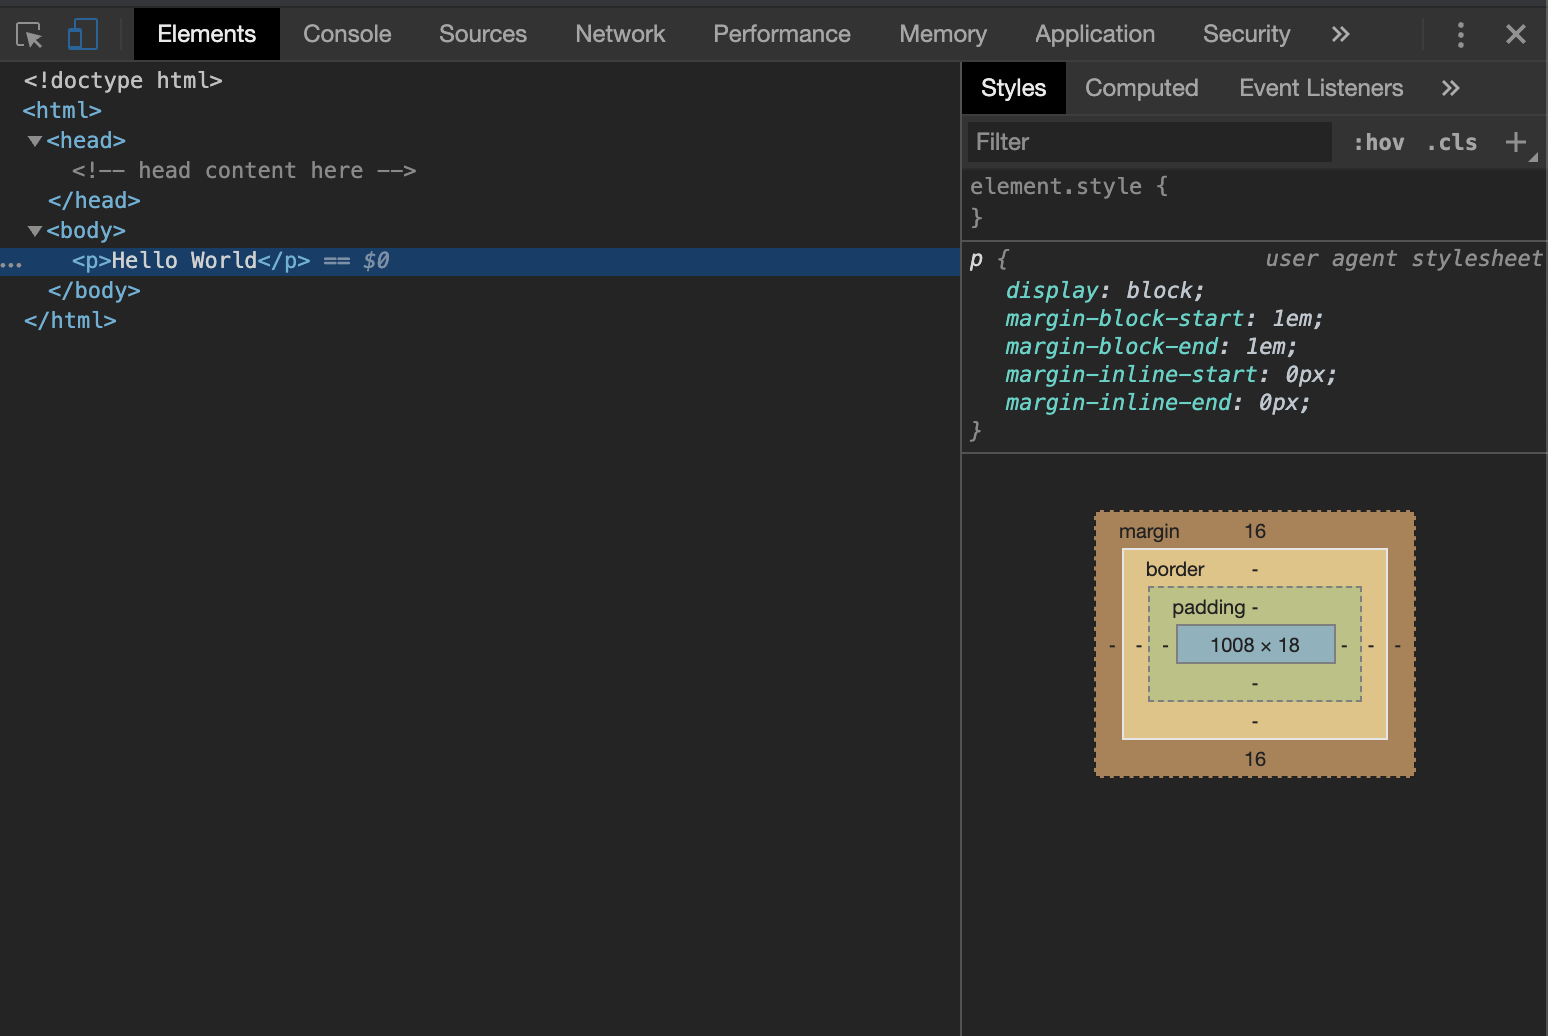
\includegraphics[width=21.5in]{images/survival-kit/dom} \caption{Inspection of the DOM in the Hello World example}\label{fig:html-dom}
\end{figure}

\hypertarget{preliminary-introduction-to-css-and-javascript}{%
\section{Preliminary introduction to CSS and JavaScript}\label{preliminary-introduction-to-css-and-javascript}}

CSS and JavaScript are tools to enhance an HTML page.

\hypertarget{html-and-css}{%
\subsection{HTML and CSS}\label{html-and-css}}

CSS (Cascading Style Sheets) changes the style of HTML tags by targeting specific classes or ids. For instance, if we want all p tags to have red color we will use:

\begin{Shaded}
\begin{Highlighting}[]
\NormalTok{p \{}
  \KeywordTok{color}\NormalTok{: }\DecValTok{red}\NormalTok{;}
\NormalTok{\}}
\end{Highlighting}
\end{Shaded}

To include CSS in an HTML page, we use the \texttt{\textless{}style\textgreater{}} tag as follows:

\begin{Shaded}
\begin{Highlighting}[]
\DataTypeTok{<!DOCTYPE }\NormalTok{HTML}\DataTypeTok{>}
\KeywordTok{<html>}
  \KeywordTok{<head>}
    \KeywordTok{<style}\OtherTok{ type=}\StringTok{"text/css"}\KeywordTok{>}
\NormalTok{      p \{}
        \KeywordTok{color}\NormalTok{: }\DecValTok{red}\NormalTok{;}
\NormalTok{      \}}
    \KeywordTok{</style>}
  \KeywordTok{</head>}
  \KeywordTok{<body>}
  \KeywordTok{<p>}\NormalTok{Hello World}\KeywordTok{</p>}
  \KeywordTok{</body>}
\KeywordTok{</html>}
\end{Highlighting}
\end{Shaded}

You may update the hello-world.html script and run it in your web-browser to see the difference (this is not super impressive but a good start). There exist other ways to include CSS (see next chapters).

\hypertarget{html-and-javascript}{%
\subsection{HTML and JavaScript}\label{html-and-javascript}}

JavaScript is also going to be one of our best friend in this book.
You will see how quickly/seamlessly you may add awesome feature to your shiny app.

Let's consider an example below:

\begin{Shaded}
\begin{Highlighting}[]
\DataTypeTok{<!DOCTYPE }\NormalTok{HTML}\DataTypeTok{>}
\KeywordTok{<html>}
  \KeywordTok{<head>}
    \KeywordTok{<style}\OtherTok{ type=}\StringTok{"text/css"}\KeywordTok{>}
\NormalTok{      p \{}
        \KeywordTok{color}\NormalTok{: }\DecValTok{red}\NormalTok{;}
\NormalTok{      \}}
    \KeywordTok{</style>}
    \KeywordTok{<script}\OtherTok{ language=}\StringTok{"javascript"}\KeywordTok{>}
      \CommentTok{// displays an alert }
      \AttributeTok{alert}\NormalTok{(}\StringTok{'Click on the Hello World text!'}\NormalTok{)}\OperatorTok{;}
      \CommentTok{// change text color}
      \KeywordTok{function} \AttributeTok{changeColor}\NormalTok{(color)}\OperatorTok{\{}
        \VariableTok{document}\NormalTok{.}\AttributeTok{getElementById}\NormalTok{(}\StringTok{'hello'}\NormalTok{).}\VariableTok{style}\NormalTok{.}\AttributeTok{color} \OperatorTok{=} \StringTok{"green"}\OperatorTok{;}
      \OperatorTok{\}}
    \KeywordTok{</script>}
  \KeywordTok{</head>}
  \KeywordTok{<body>}
    \CommentTok{<!-- onclick attributes applies the JavaScript function changeColor define above -->}
    \KeywordTok{<p}\OtherTok{ id=}\StringTok{"hello"}\OtherTok{ onclick=}\StringTok{"changeColor('green')"}\KeywordTok{>}\NormalTok{Hello World}\KeywordTok{</p>}
  \KeywordTok{</body>}
\KeywordTok{</html>}
\end{Highlighting}
\end{Shaded}

In few lines of code, you can change the color of the text. Wonderful isn'it?
Let's move to the next chapter to discover JavaScript!

\hypertarget{survival-kit-javascript}{%
\chapter{JavaScript}\label{survival-kit-javascript}}

\hypertarget{introduction}{%
\section{Introduction}\label{introduction}}

JavaScript (JS) was created in 1995 by Brendan Eich and also known as ECMAScript (ES). Interestingly, you might have heard about ActionScript, which is no more than an implementation of ES by Adobe Systems. Nowadays, JavaScript is a centerpiece of the web and included in almost all websites.

Let's make a little experiment. If you have a personal blog (it is very popular in the RStats community) you probably know Hugo or Jekyll. These tools allow to quickly setup professionnal looking (or at least not too ugly) blogs in literraly few minutes. You can focus on the content and this is what matters! Now, if you open the HTML inspector introduced in Chapter \ref{survival-kit-html}, click on the elements tab (in theory it is the first tab and open by default), and uncollapse the \texttt{\textless{}head\textgreater{}} tag, you see that a lot of scripts are included, as shown in Figure \ref{fig:scripts-list}. Same remark in the \texttt{\textless{}body\textgreater{}} tag.

\begin{figure}
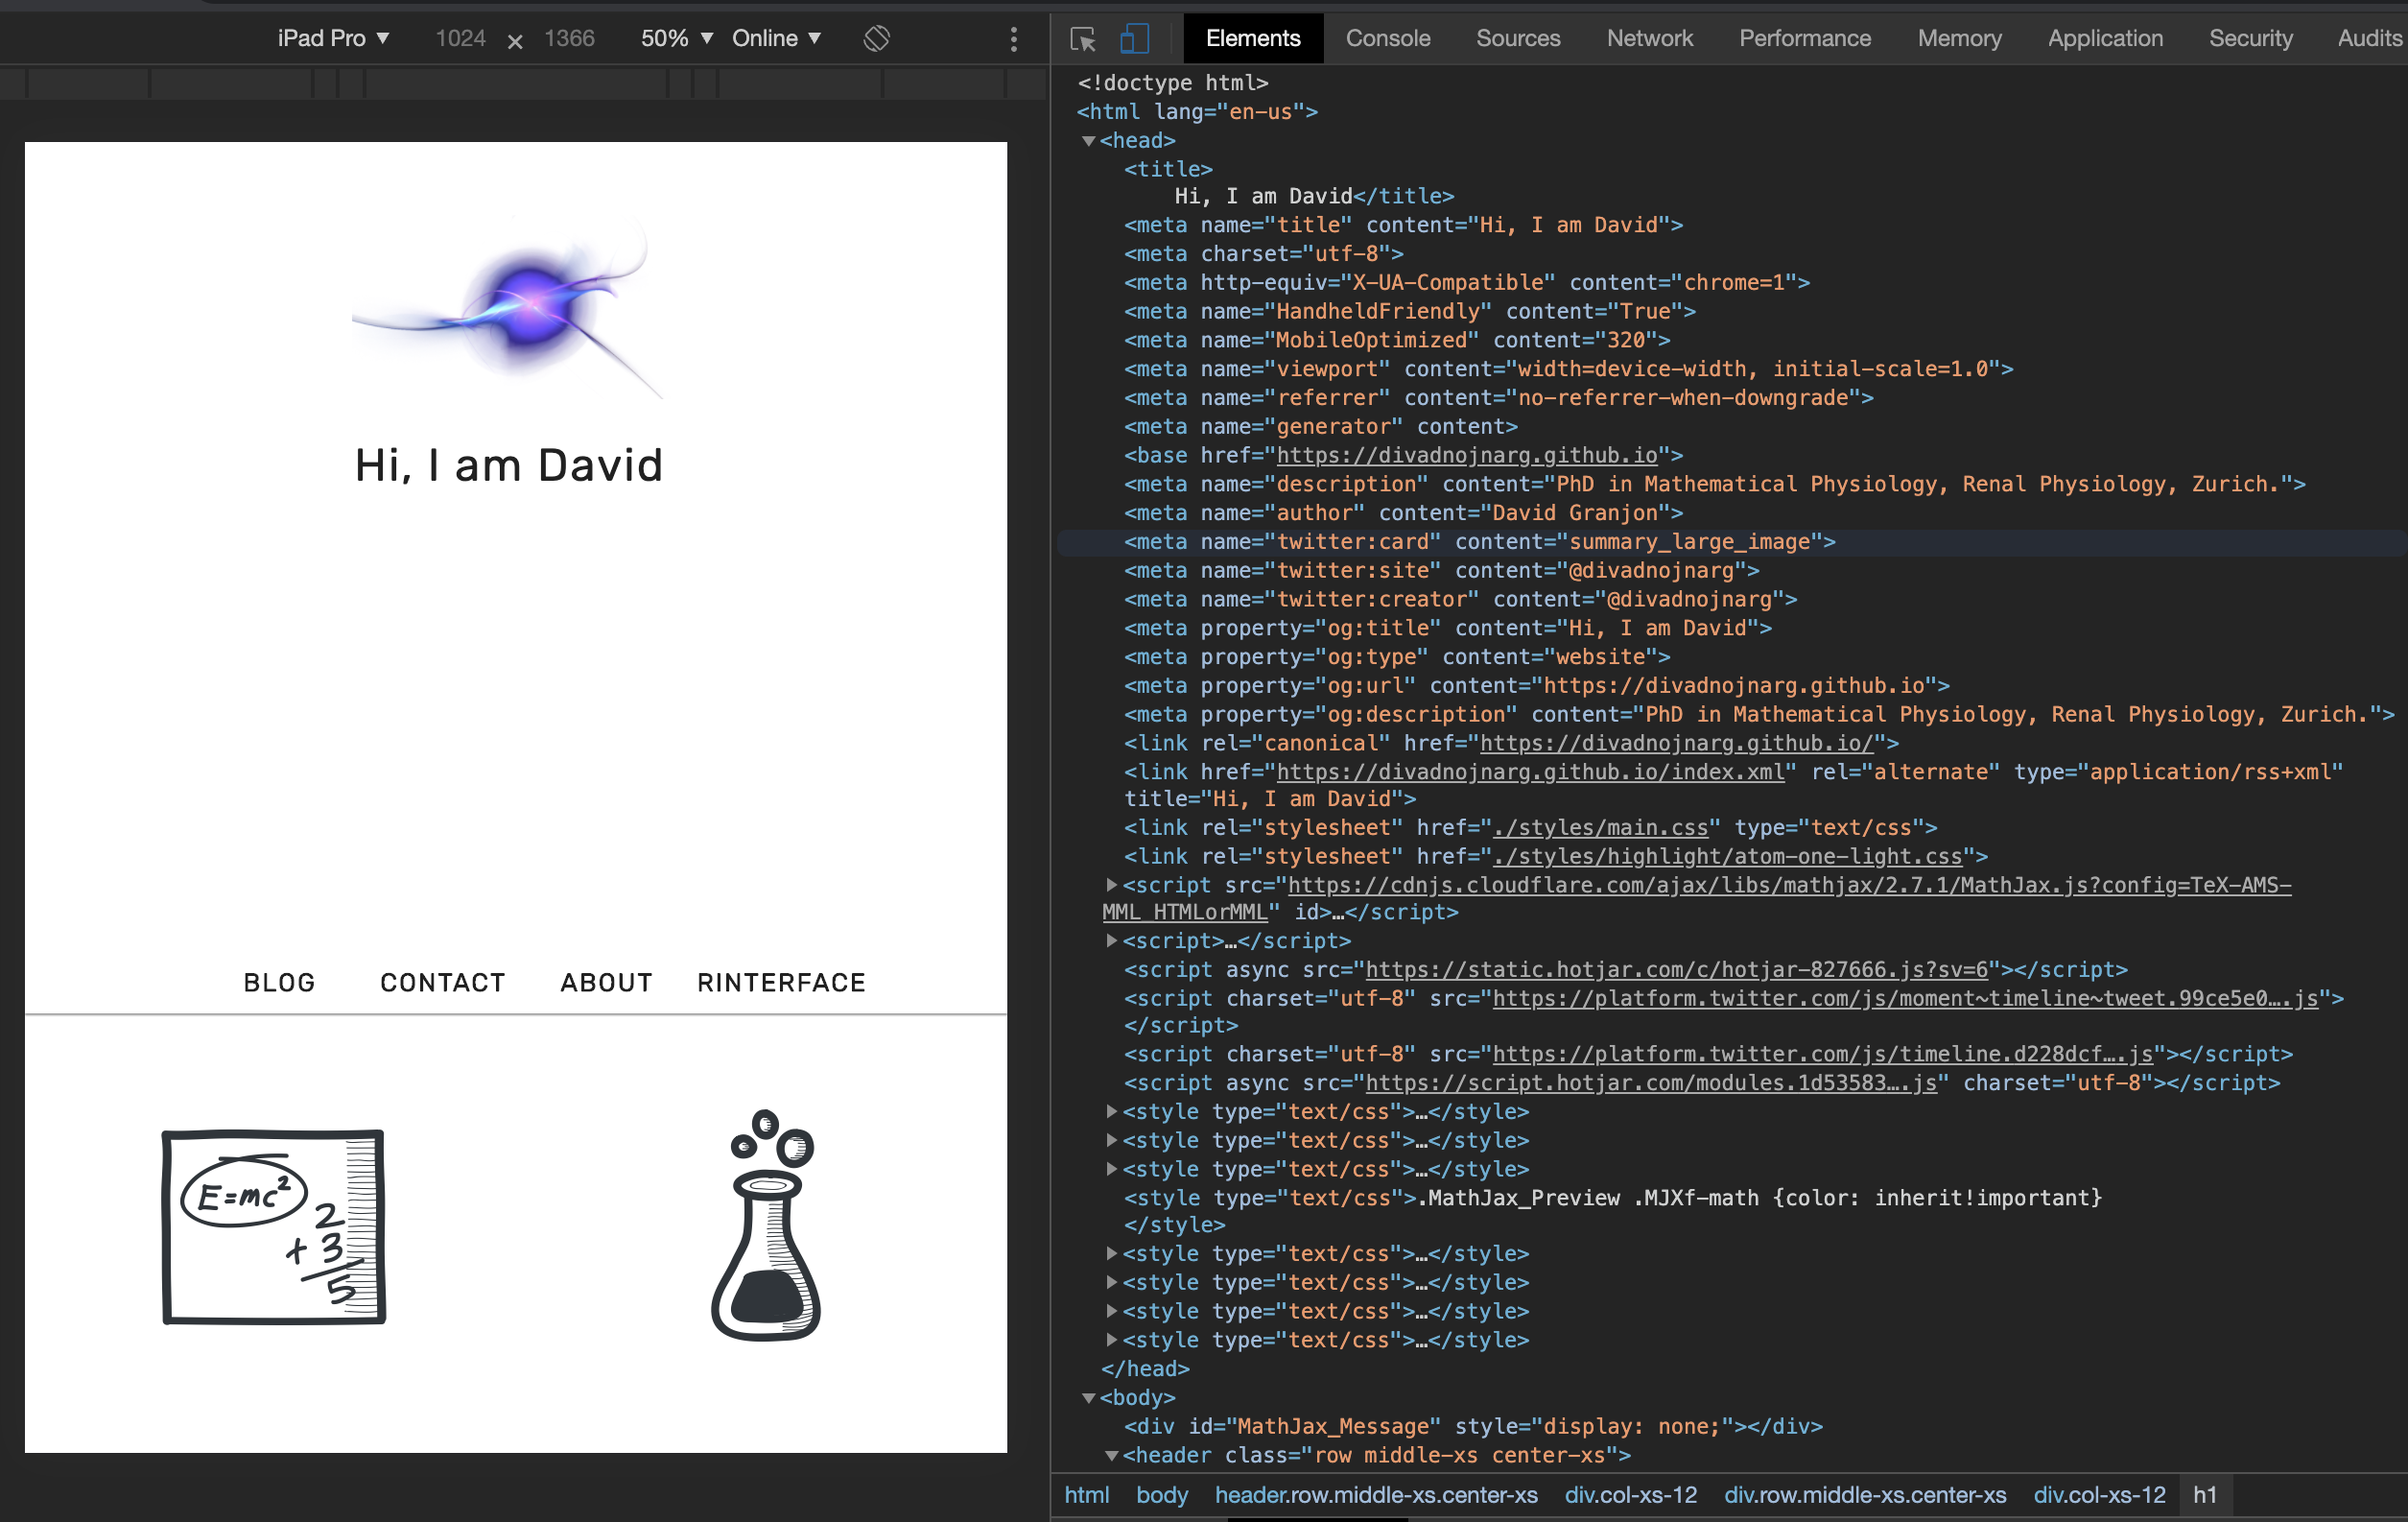
\includegraphics[width=34.86in]{images/survival-kit/scripts-list} \caption{A website is full of JavaScript}\label{fig:scripts-list}
\end{figure}

There are 2 ways to include scripts:

\begin{itemize}
\tightlist
\item
  Use the \texttt{\textless{}script\textgreater{}} tag with the JS code inside
\item
  Import an external file containing the JS code and only
\end{itemize}

\begin{Shaded}
\begin{Highlighting}[]
\KeywordTok{<script}\OtherTok{ type=}\StringTok{"text/javascript"}\KeywordTok{>}
\CommentTok{// JS code here}
\KeywordTok{</script>}
\end{Highlighting}
\end{Shaded}

\begin{Shaded}
\begin{Highlighting}[]
\CommentTok{<!-- We use the src attribute to link the external file -->}
\KeywordTok{<script}\OtherTok{ type=}\StringTok{"text/javascript"}\OtherTok{ src=}\StringTok{"file.js"}\KeywordTok{>}
\end{Highlighting}
\end{Shaded}

Whether to choose the first or second method depends on the content of your script. If we consider jQuery, a well known JS library, it contains so much lines of code that it does not make sense to select the first method.

\hypertarget{setup}{%
\section{Setup}\label{setup}}

Like R or Python, JavaScript is an interpreted language. It is also executed client side, that is in the navigator. It also means that you cannot run js code without suitable tools.

\hypertarget{node}{%
\subsection{Node}\label{node}}

\href{https://nodejs.org/en/}{Node} contains an interpreter for JS as well as a dependencies manager, npm (Node Package Manager). To install Node on your computer, browse to the website and follow the intruction. Once done, open a terminal and check if

\begin{verbatim}
$ which node
$ node --version
\end{verbatim}

returns something. If not, it means that Node is not properly installed.

\hypertarget{choose-a-good-ide}{%
\subsection{Choose a good IDE}\label{choose-a-good-ide}}

I really like \href{https://code.visualstudio.com}{VSCode} for all the JS things since it contains a Node interpreter and you can seamlessly execute any JS code (the truth is because I'm a big fan of the dracula color theme). But the \href{https://rstudio.com/products/rstudio/}{Rstudio IDE} may also be fine, provided that you have Node installed. Below, we will see how to run a JS code in both IDE.

\hypertarget{first-script}{%
\subsection{First Script}\label{first-script}}

Let's write our first script:

\begin{Shaded}
\begin{Highlighting}[]
\VariableTok{console}\NormalTok{.}\AttributeTok{log}\NormalTok{(}\StringTok{"Hello World"}\NormalTok{)}\OperatorTok{;}
\end{Highlighting}
\end{Shaded}

You notice that all instruction end by \texttt{;}. You can run this script either in Rstudio IDE or VSCode.

\begin{figure}
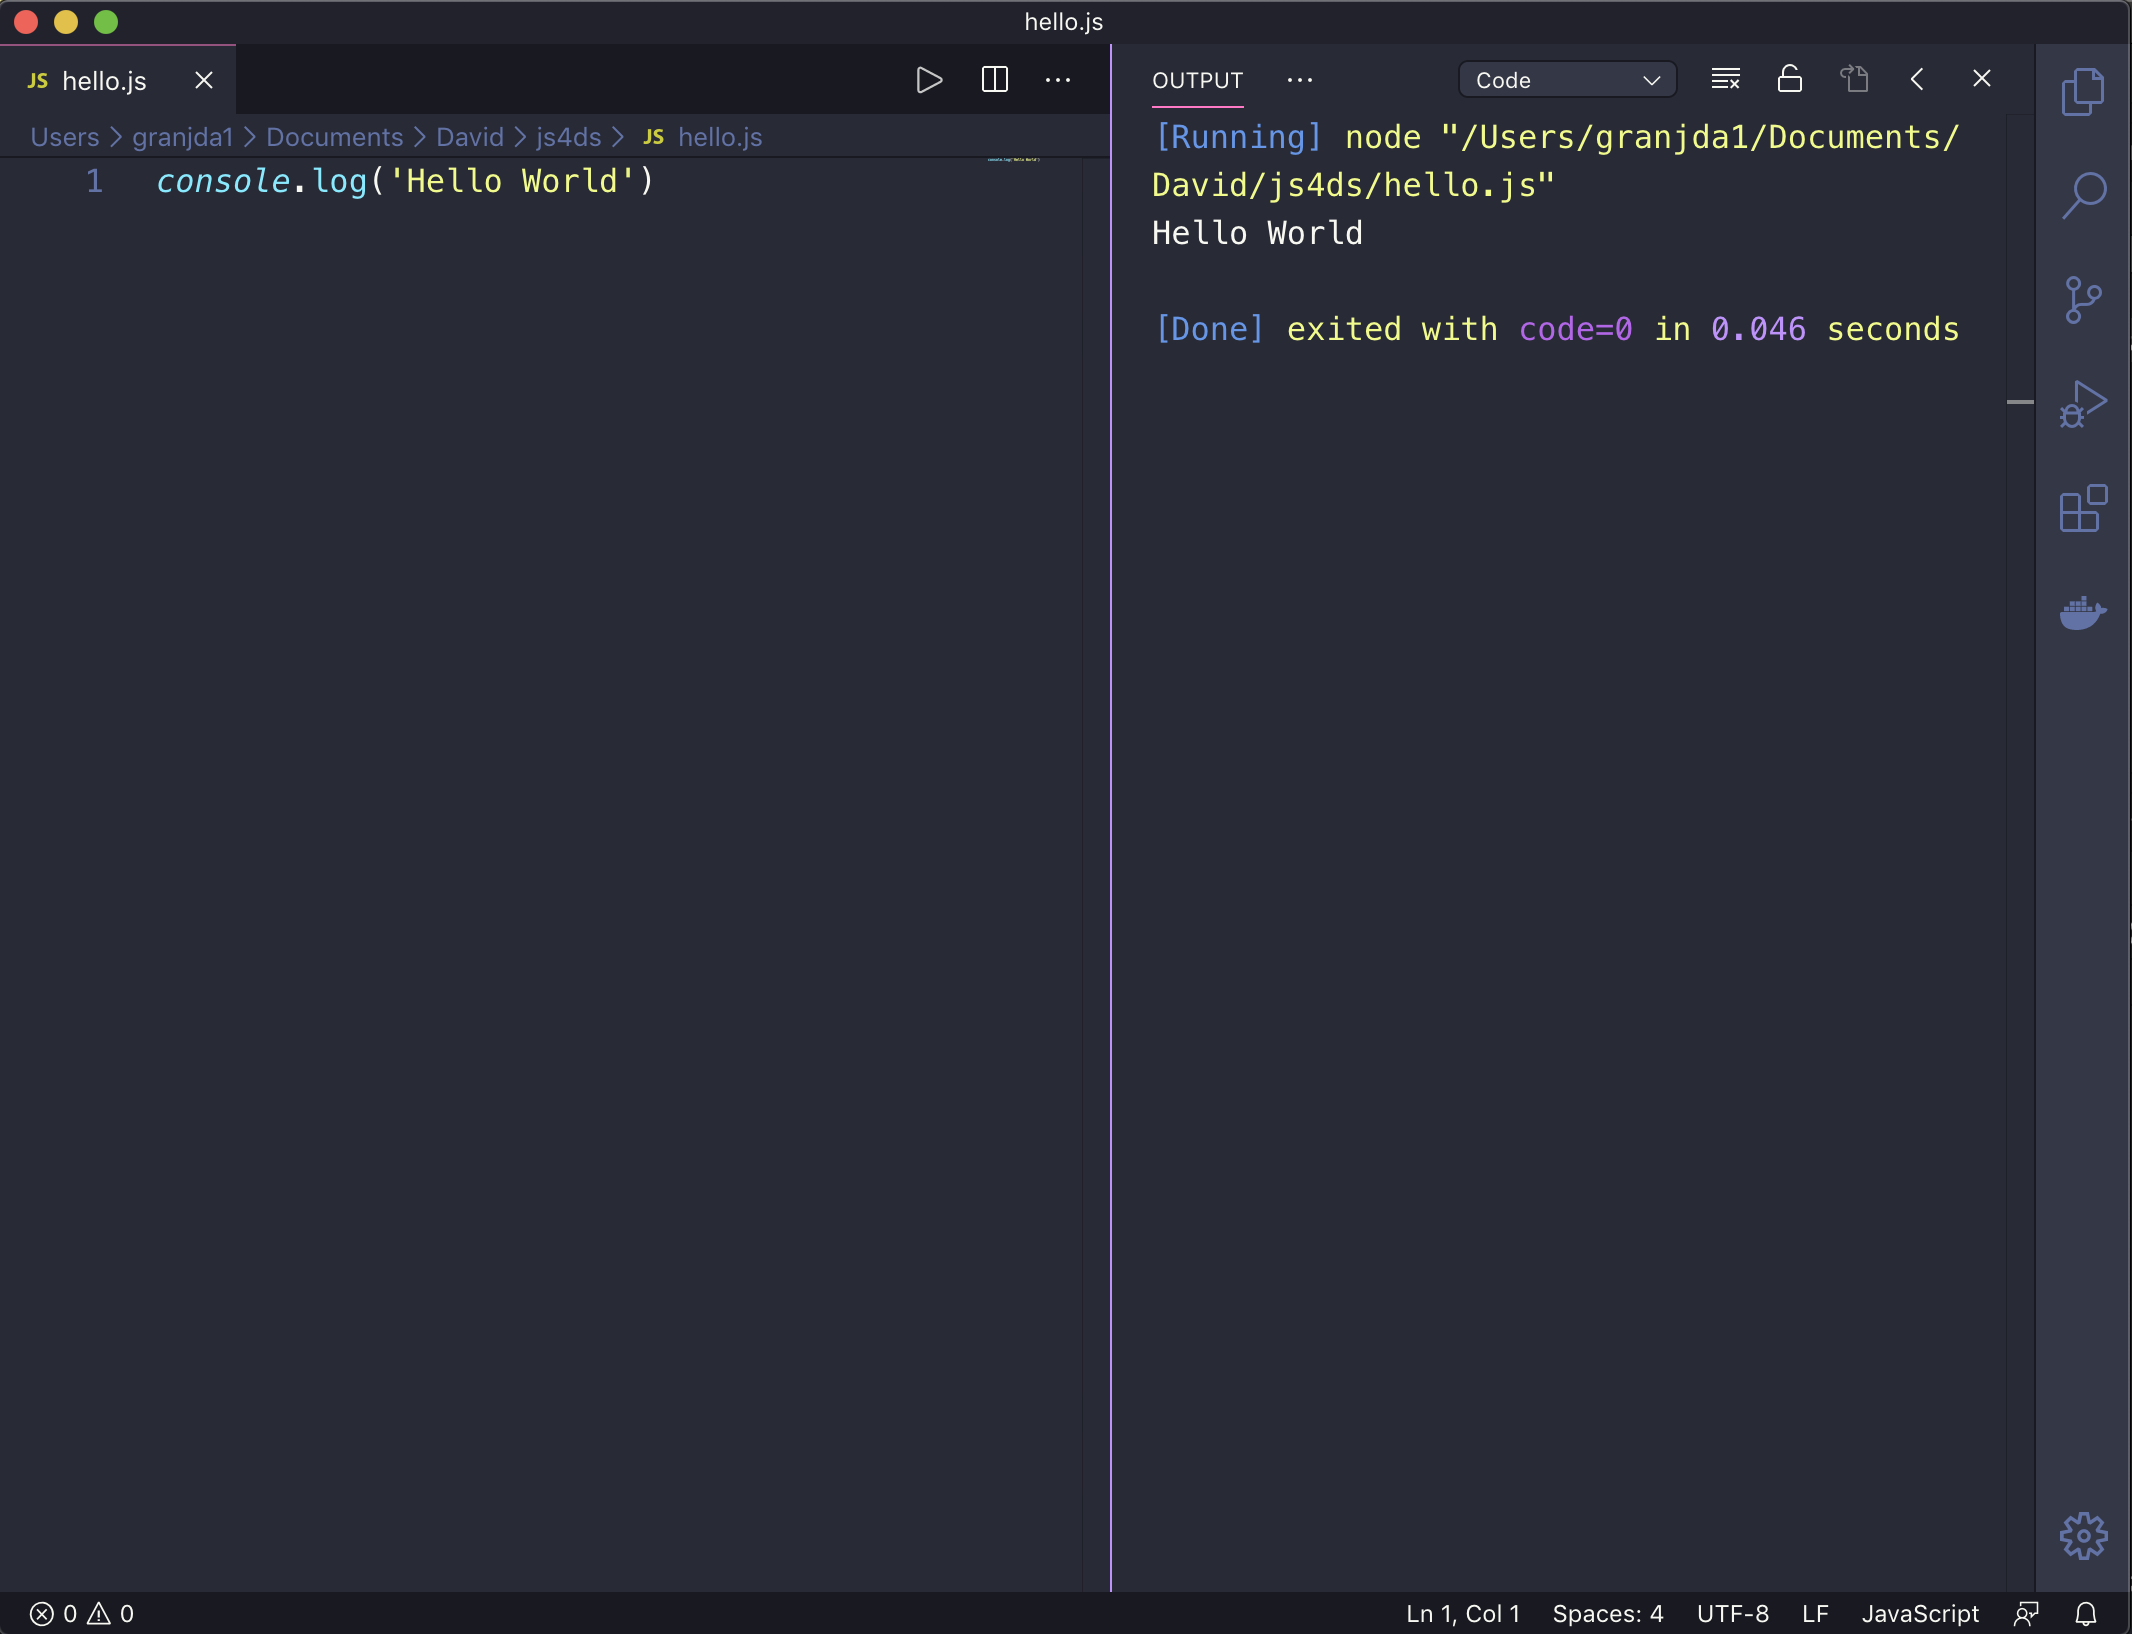
\includegraphics[width=29.61in]{images/survival-kit/script-vscode} \caption{Run JS in VSCode}\label{fig:script-vscode}
\end{figure}

In VSCode, clicking on the run arrow (top center) of Figure \ref{fig:script-vscode},
triggers the \texttt{node\ hello.js} command, which tells Node to run my script. We see the result in the right panel (code=0 means the execution is fine and we even have the compute time). To run this script in the RStudio IDE, you need to click on the terminal tab (you could also open a basic terminal) and type \texttt{node\ hello.js} (or \texttt{node\ mycustompath/hello.js} if you are not in the folder containing the script). You should see the Hello World message in the console (see Figure \ref{fig:script-rstudio}).

\begin{figure}
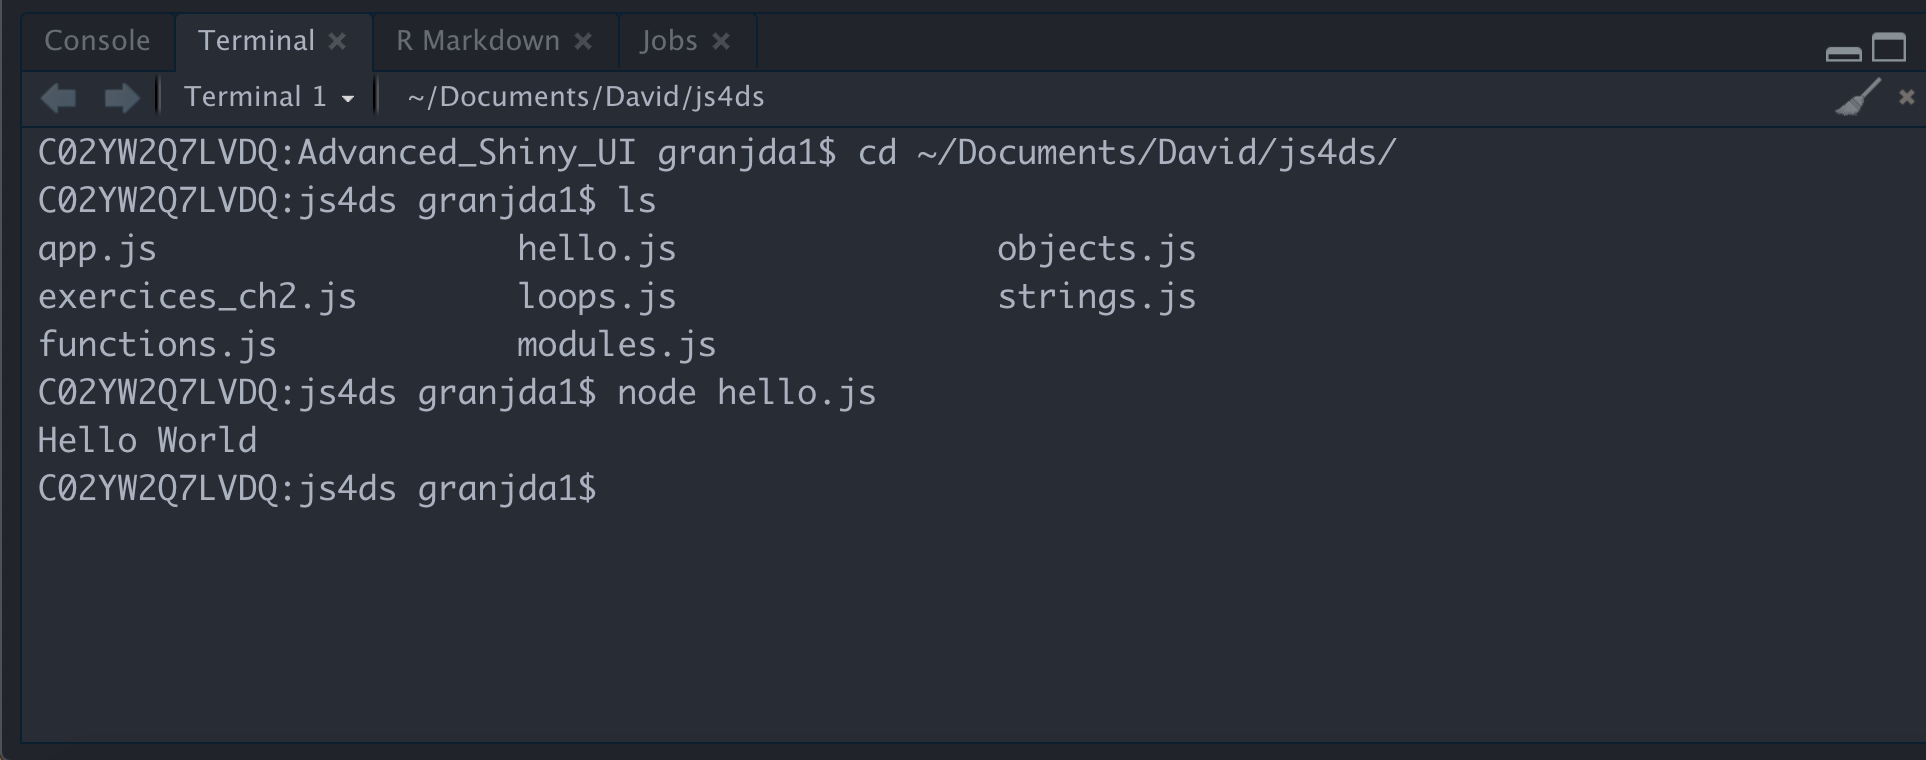
\includegraphics[width=26.75in]{images/survival-kit/script-rstudio} \caption{Run JS in a terminal}\label{fig:script-rstudio}
\end{figure}

\hypertarget{programming-with-js-basis}{%
\section{Programming with JS: basis}\label{programming-with-js-basis}}

We are now all set to introduce the basis of JS. As many languages, JS is made of variables and instructions (We saw above that instructions end by \texttt{;}).

\hypertarget{js-types}{%
\subsection{JS types}\label{js-types}}

JS defines several types:

\begin{itemize}
\tightlist
\item
  Number: does not distinguish between integers and others (in R for instance, numeric contains integers and double)
\item
  String: characters (`blabla')
\item
  Boolean: true/false
\end{itemize}

To check the type of an element, we may use the \texttt{typeof} operator (this is not a function like the \texttt{typeof} function in R).

\begin{Shaded}
\begin{Highlighting}[]
\KeywordTok{typeof} \DecValTok{1}\OperatorTok{;} \CommentTok{// number}
\KeywordTok{typeof} \StringTok{'pouic'}\OperatorTok{;} \CommentTok{// string}
\end{Highlighting}
\end{Shaded}

\hypertarget{variables}{%
\subsection{Variables}\label{variables}}

A variable is defined by:

\begin{itemize}
\tightlist
\item
  a type
\item
  a name
\item
  a value
\end{itemize}

Valid variable names:

don't use an existing name like typeof

son't start with a number (123)

don't include any space (total price)

Based on the above forbidden items, you can use the camelCase syntax to write your variables in JS. To set a variable we use \texttt{let} (there exists \texttt{var} but this is not the latest JS norm (ES6). You will see later that we still use \texttt{var} in the shiny core and many other R packages):

\begin{Shaded}
\begin{Highlighting}[]
\KeywordTok{let}\NormalTok{ myVariable }\OperatorTok{=} \StringTok{'welcome'}\OperatorTok{;}
\VariableTok{console}\NormalTok{.}\AttributeTok{log}\NormalTok{(myVariable)}\OperatorTok{;}
\end{Highlighting}
\end{Shaded}

Then we can use all mathematical operators to manipulate a variable.

\begin{Shaded}
\begin{Highlighting}[]
\KeywordTok{let}\NormalTok{ myNumber }\OperatorTok{=} \DecValTok{1}\OperatorTok{;} \CommentTok{// affectation}
\NormalTok{myNumber}\OperatorTok{--;} \CommentTok{// decrement}
\VariableTok{console}\NormalTok{.}\AttributeTok{log}\NormalTok{(myNumber)}\OperatorTok{;} \CommentTok{// print 0}
\end{Highlighting}
\end{Shaded}

List of numerical operators in JS:

+

-

*

/

\% (modulo)

++ (incrementation)

-- (decrementation)

To concatenate 2 strings, use \texttt{+}.

\hypertarget{conditions}{%
\subsection{Conditions}\label{conditions}}

Below are the operators to check conditions.

== (A equal B)

!= (A not equal to B)

\begin{quote}
(\textgreater{}=)

\textless{} (\textless{}=)

AND (A AND B)

OR (A OR B)
\end{quote}

To test conditions there exists several ways:

\begin{itemize}
\tightlist
\item
  \texttt{if\ (condition)\ \{\ console.log(\textquotesingle{}Test\ passed\textquotesingle{});\ \}}
\item
  \texttt{if\ (condition)\ \{\ instruction\ A\}\ else\ \{\ instruction\ B\ \}}
\end{itemize}

This is very common to other languages (and R for instance). Whenever a lot of possible conditions need to be evaluated, it is better to choose the \texttt{switch}.

\begin{Shaded}
\begin{Highlighting}[]
\ControlFlowTok{switch}\NormalTok{ (variable) }\OperatorTok{\{}
  \ControlFlowTok{case} \DataTypeTok{val1}\OperatorTok{:} \CommentTok{// instruction 1}
  \ControlFlowTok{break}\OperatorTok{;} \CommentTok{// don't forget the break!}
  \ControlFlowTok{case} \DataTypeTok{val2}\OperatorTok{:}  \CommentTok{// instruction 2}
  \ControlFlowTok{break}\OperatorTok{;}
  \DataTypeTok{default}\OperatorTok{:} \CommentTok{// when none of val1 and val2 are satisfied}
\OperatorTok{\}}
\end{Highlighting}
\end{Shaded}

\hypertarget{iterations}{%
\subsection{Iterations}\label{iterations}}

\hypertarget{survival-kit-shiny}{%
\chapter{Shiny}\label{survival-kit-shiny}}

\hypertarget{part-htmltools}{%
\part*{htmltools}\label{part-htmltools}}
\addcontentsline{toc}{part}{htmltools}

While building a custom html template, you will need to know more about the wonderful \href{https://github.com/rstudio/htmltools}{htmltools} developed by Winston Chang, member of the shiny core team. It has the same spirit as devtools, that is, making your web developer life easier. What follows does not have the pretention to be an exhaustive guide about this package. Yet, it will provide you yith the main tools to be more efficient.

\hypertarget{htmltools-overview}{%
\chapter{htmltools overview}\label{htmltools-overview}}

\hypertarget{html-tags}{%
\section{HTML Tags}\label{html-tags}}

htmltools contains tools to write HTML tags we saw in Chapter \ref{survival-kit-html}:

\begin{Shaded}
\begin{Highlighting}[]
\KeywordTok{div}\NormalTok{()}
\end{Highlighting}
\end{Shaded}

If you had to gather multiple tags together, prefer \texttt{tagList()} as \texttt{list()}, although the HTML output is the same. The first has the shiny.tag.list class in addition to list. (The \href{http://golemverse.org}{Golem} package allows to test if a R object is a tag list, therefore using list would make the test fail).

\hypertarget{notations}{%
\section{Notations}\label{notations}}

Whether to use \texttt{tags\$div} or \texttt{div} depends if the tag is exported by default.
For instance, you could use \texttt{htmltools::div} but not \texttt{htmltools::nav} since nav does not have a dedicated function (only for p, h1, h2, h3, h4, h5, h6, a, br, div, span, pre, code, img, strong, em, hr).
Rather use \texttt{htmltools::tags\$nav}. Alternatively, there exists a function (in shiny and htmltools)
called \texttt{withTags()}. Wrapping your code in this function enables you to use \texttt{withTags(nav(),\ ...)}
instead of \texttt{tags\$nav()}.

\hypertarget{adding-new-tags}{%
\section{Adding new tags}\label{adding-new-tags}}

The \texttt{tag} function allows to add extra HTML tags not already defined. You may use it as follows:

\begin{Shaded}
\begin{Highlighting}[]
\KeywordTok{tag}\NormalTok{(}\StringTok{"test"}\NormalTok{, }\KeywordTok{list}\NormalTok{(}\DataTypeTok{class =} \StringTok{"test"}\NormalTok{, }\KeywordTok{p}\NormalTok{(}\StringTok{"Custom Tag"}\NormalTok{)))}
\CommentTok{# structure below}
\NormalTok{█─tag }
\NormalTok{├─}\StringTok{"test"} 
\NormalTok{└─█─list }
\NormalTok{├─class =}\StringTok{ "test"} 
\NormalTok{└─█─p }
\NormalTok{└─}\StringTok{"Custom Tag"} 
\end{Highlighting}
\end{Shaded}

\hypertarget{alternative-way-to-write-tags}{%
\section{Alternative way to write tags}\label{alternative-way-to-write-tags}}

htmltools comes with the \texttt{HTML()} function that you can feed with raw HTML:

\begin{Shaded}
\begin{Highlighting}[]
\KeywordTok{HTML}\NormalTok{(}\StringTok{'<div>Blabla</div>'}\NormalTok{)}
\CommentTok{# will render exactly like}
\KeywordTok{div}\NormalTok{(}\StringTok{"Blabla"}\NormalTok{)}

\CommentTok{# but there class is different}
\KeywordTok{class}\NormalTok{(}\KeywordTok{HTML}\NormalTok{(}\StringTok{'<div>Blabla</div>'}\NormalTok{))}
\KeywordTok{class}\NormalTok{(}\KeywordTok{div}\NormalTok{(}\StringTok{"Blabla"}\NormalTok{))}
\end{Highlighting}
\end{Shaded}

You will not be able to use tag related functions, as in the following parts.
Therefore, I strongly recommand using R and not mixing HTML in R. Interestingly, if
you want to convert HTML to R code, there is a Shiny App developed by Alan
Dipert from RStudio, namely \href{https://github.com/alandipert/html2r}{html2R}. There
are some issues, non standard attributes (like \texttt{data-toggle}) are not correctly processed but there are \href{https://github.com/alandipert/html2r/issues/2}{fixes}. This will save you precious time!

\hypertarget{playing-with-tags}{%
\section{Playing with tags}\label{playing-with-tags}}

\hypertarget{tags-structure}{%
\subsection{Tags structure}\label{tags-structure}}

According to the \texttt{tag} function, a tag has:

\begin{itemize}
\tightlist
\item
  a name such as span, div, h1 \ldots{} \texttt{tag\$name}
\item
  some attributes, which you can access with \texttt{tag\$attribs}
\item
  children, which you can access with \texttt{tag\$children}
\item
  a class, namely ``shiny.tag''
\end{itemize}

For instance:

\begin{Shaded}
\begin{Highlighting}[]
\CommentTok{# create the tag}
\NormalTok{myTag <-}\StringTok{ }\KeywordTok{div}\NormalTok{(}
  \DataTypeTok{class =} \StringTok{"divclass"}\NormalTok{, }
  \DataTypeTok{id =} \StringTok{"first"}\NormalTok{,}
  \KeywordTok{h1}\NormalTok{(}\StringTok{"Here comes your baby"}\NormalTok{),}
  \KeywordTok{span}\NormalTok{(}\DataTypeTok{class =} \StringTok{"child"}\NormalTok{, }\DataTypeTok{id =} \StringTok{"baby"}\NormalTok{, }\StringTok{"Crying"}\NormalTok{)}
\NormalTok{)}
\CommentTok{# access its name}
\NormalTok{myTag}\OperatorTok{$}\NormalTok{name}
\CommentTok{# access its attributes (id and class)}
\NormalTok{myTag}\OperatorTok{$}\NormalTok{attribs}
\CommentTok{# access children (returns a list of 2 elements)}
\NormalTok{myTag}\OperatorTok{$}\NormalTok{children}
\CommentTok{# access its class}
\KeywordTok{class}\NormalTok{(myTag)}
\end{Highlighting}
\end{Shaded}

How to modify the class of the second child, namely span?

\begin{Shaded}
\begin{Highlighting}[]
\NormalTok{second_children <-}\StringTok{ }\NormalTok{myTag}\OperatorTok{$}\NormalTok{children[[}\DecValTok{2}\NormalTok{]]}
\NormalTok{second_children}\OperatorTok{$}\NormalTok{attribs}\OperatorTok{$}\NormalTok{class <-}\StringTok{ "adult"}
\NormalTok{myTag}
\CommentTok{# Hummm, this is not working ...}
\end{Highlighting}
\end{Shaded}

Why is this not working? By assigning \texttt{myTag\$children{[}{[}2{]}{]}} to second\_children, \texttt{second\_children\$attribs\$class\ \textless{}-\ "adult"} modifies the class of the copy and not the original object. Thus we do:

\begin{Shaded}
\begin{Highlighting}[]
\NormalTok{myTag}\OperatorTok{$}\NormalTok{children[[}\DecValTok{2}\NormalTok{]]}\OperatorTok{$}\NormalTok{attribs}\OperatorTok{$}\NormalTok{class <-}\StringTok{ "adult"}
\NormalTok{myTag}
\end{Highlighting}
\end{Shaded}

In the following section we explore helper functions, such as \texttt{tagAppendChild} from htmltools.

\hypertarget{useful-functions-for-tags}{%
\subsection{Useful functions for tags}\label{useful-functions-for-tags}}

htmltools and Shiny have powerful functions to easily add attributes to tags, check for existing attributes, get attributes and add other siblings to a list of tags.

\hypertarget{add-attributes}{%
\subsubsection{Add attributes}\label{add-attributes}}

\begin{itemize}
\tightlist
\item
  \texttt{tagAppendAttributes}: this function allow you to add a new attribute to the current tag.
\end{itemize}

For instance, assuming you created a div for which you forgot to add an id attribute:

\begin{Shaded}
\begin{Highlighting}[]
\NormalTok{mydiv <-}\StringTok{ }\KeywordTok{div}\NormalTok{(}\StringTok{"Where is my brain"}\NormalTok{)}
\NormalTok{mydiv <-}\StringTok{ }\KeywordTok{tagAppendAttributes}\NormalTok{(mydiv, }\DataTypeTok{id =} \StringTok{"here_it_is"}\NormalTok{)}
\end{Highlighting}
\end{Shaded}

You can pass as many attributes as you want, including non standard attributes such as \texttt{data-toggle} (see Bootstrap 3 tabs for instance):

\begin{Shaded}
\begin{Highlighting}[]
\NormalTok{mydiv <-}\StringTok{ }\KeywordTok{tagAppendAttributes}\NormalTok{(mydiv, }\StringTok{`}\DataTypeTok{data-toggle}\StringTok{`}\NormalTok{ =}\StringTok{ "tabs"}\NormalTok{)}
\CommentTok{# even though you could proceed as follows}
\NormalTok{mydiv}\OperatorTok{$}\NormalTok{attribs[[}\StringTok{"aria-controls"}\NormalTok{]] <-}\StringTok{ "home"}
\end{Highlighting}
\end{Shaded}

\hypertarget{check-if-tag-has-specific-attribute}{%
\subsubsection{Check if tag has specific attribute}\label{check-if-tag-has-specific-attribute}}

\begin{itemize}
\tightlist
\item
  \texttt{tagHasAttribute}: to check if a tag has a specific attribute
\end{itemize}

\begin{Shaded}
\begin{Highlighting}[]
\CommentTok{# I want to know if div has a class}
\NormalTok{mydiv <-}\StringTok{ }\KeywordTok{div}\NormalTok{(}\DataTypeTok{class =} \StringTok{"myclass"}\NormalTok{)}
\NormalTok{has_class <-}\StringTok{ }\KeywordTok{tagHasAttribute}\NormalTok{(mydiv, }\StringTok{"class"}\NormalTok{)}
\NormalTok{has_class}
\CommentTok{# if you are familiar with %>%}
\NormalTok{has_class <-}\StringTok{ }\NormalTok{mydiv }\OperatorTok\StringTok{ }\KeywordTok{tagHasAttribute}\NormalTok{(}\StringTok{"class"}\NormalTok{)}
\NormalTok{has_class}
\end{Highlighting}
\end{Shaded}

\hypertarget{get-all-attributes}{%
\subsubsection{Get all attributes}\label{get-all-attributes}}

\begin{itemize}
\tightlist
\item
  \texttt{tagGetAttribute}: to get the value of the targeted attributes, if it exists, otherwise NULL.
\end{itemize}

\begin{Shaded}
\begin{Highlighting}[]
\NormalTok{mydiv <-}\StringTok{ }\KeywordTok{div}\NormalTok{(}\DataTypeTok{class =} \StringTok{"test"}\NormalTok{)}
\CommentTok{# returns the class}
\KeywordTok{tagGetAttribute}\NormalTok{(mydiv, }\StringTok{"class"}\NormalTok{)}
\CommentTok{# returns NULL}
\KeywordTok{tagGetAttribute}\NormalTok{(mydiv, }\StringTok{"id"}\NormalTok{)}
\end{Highlighting}
\end{Shaded}

\hypertarget{set-childchildren}{%
\subsubsection{Set child/children}\label{set-childchildren}}

\begin{itemize}
\tightlist
\item
  \texttt{tagSetChildren} allows to create children for a given tag. For instance:
\end{itemize}

\begin{Shaded}
\begin{Highlighting}[]
\NormalTok{mydiv <-}\StringTok{ }\KeywordTok{div}\NormalTok{(}\DataTypeTok{class =} \StringTok{"parent"}\NormalTok{, }\DataTypeTok{id =} \StringTok{"mother"}\NormalTok{, }\StringTok{"Not the mama!!!"}\NormalTok{)}
\CommentTok{# mydiv has 1 child "Not the mama!!!"}
\NormalTok{mydiv }
\NormalTok{children <-}\StringTok{ }\KeywordTok{lapply}\NormalTok{(}\DecValTok{1}\OperatorTok{:}\DecValTok{3}\NormalTok{, span)}
\NormalTok{mydiv <-}\StringTok{ }\KeywordTok{tagSetChildren}\NormalTok{(mydiv, children)}
\CommentTok{# mydiv has 3 children, the first one was removed}
\NormalTok{mydiv }
\end{Highlighting}
\end{Shaded}

Notice that \texttt{tagSetChildren} removes all existing children. Below we see another set of functions to add children while conserving existing ones.

\hypertarget{add-child-or-children}{%
\subsubsection{Add child or children}\label{add-child-or-children}}

\begin{itemize}
\tightlist
\item
  \texttt{tagAppendChild} and \texttt{tagAppendChildren}: add other tags to an existing tag.
  Whereas \texttt{tagAppendChild} only takes one tag, you can pass a list of tags to \texttt{tagAppendChildren}.
\end{itemize}

\begin{Shaded}
\begin{Highlighting}[]
\NormalTok{mydiv <-}\StringTok{ }\KeywordTok{div}\NormalTok{(}\DataTypeTok{class =} \StringTok{"parent"}\NormalTok{, }\DataTypeTok{id =} \StringTok{"mother"}\NormalTok{, }\StringTok{"Not the mama!!!"}\NormalTok{)}
\NormalTok{otherTag <-}\StringTok{ }\KeywordTok{span}\NormalTok{(}\StringTok{"I am your child"}\NormalTok{)}
\NormalTok{mydiv <-}\StringTok{ }\KeywordTok{tagAppendChild}\NormalTok{(mydiv, otherTag)}
\end{Highlighting}
\end{Shaded}

You might wonder why there is no \texttt{tagRemoveChild} or \texttt{tagRemoveAttributes}.
Let's look at the \texttt{tagAppendChild}

\begin{Shaded}
\begin{Highlighting}[]
\NormalTok{tagAppendChild <-}\StringTok{ }\ControlFlowTok{function}\NormalTok{ (tag, child) \{}
\NormalTok{  tag}\OperatorTok{$}\NormalTok{children[[}\KeywordTok{length}\NormalTok{(tag}\OperatorTok{$}\NormalTok{children) }\OperatorTok{+}\StringTok{ }\DecValTok{1}\NormalTok{]] <-}\StringTok{ }\NormalTok{child}
\NormalTok{  tag}
\NormalTok{\}}
\end{Highlighting}
\end{Shaded}

Below we write the \texttt{tagRemoveChild}, where tag is the target and n is the position to remove in the list of children:

\begin{Shaded}
\begin{Highlighting}[]
\NormalTok{mydiv <-}\StringTok{ }\KeywordTok{div}\NormalTok{(}\DataTypeTok{class =} \StringTok{"parent"}\NormalTok{, }\DataTypeTok{id =} \StringTok{"mother"}\NormalTok{, }\StringTok{"Not the mama!!!"}\NormalTok{, }\KeywordTok{span}\NormalTok{(}\StringTok{"Hey!"}\NormalTok{))}

\CommentTok{# we create the tagRemoveChild function}
\NormalTok{tagRemoveChild <-}\StringTok{ }\ControlFlowTok{function}\NormalTok{(tag, n) \{}
  \CommentTok{# check if the list is empty}
  \ControlFlowTok{if}\NormalTok{ (}\KeywordTok{length}\NormalTok{(tag}\OperatorTok{$}\NormalTok{children) }\OperatorTok{==}\StringTok{ }\DecValTok{0}\NormalTok{) \{}
    \KeywordTok{stop}\NormalTok{(}\KeywordTok{paste}\NormalTok{(tag}\OperatorTok{$}\NormalTok{name, }\StringTok{"does not have any children!"}\NormalTok{))}
\NormalTok{  \}}
\NormalTok{  tag}\OperatorTok{$}\NormalTok{children[n] <-}\StringTok{ }\OtherTok{NULL}
\NormalTok{  tag}
\NormalTok{\}}
\NormalTok{mydiv <-}\StringTok{ }\KeywordTok{tagRemoveChild}\NormalTok{(mydiv, }\DecValTok{1}\NormalTok{)}
\NormalTok{mydiv}
\end{Highlighting}
\end{Shaded}

When defining the \texttt{tagRemoveChild}, we choose \texttt{{[}} instead of \texttt{{[}{[}} to allow to select multiple list elements:

\begin{Shaded}
\begin{Highlighting}[]
\NormalTok{mydiv <-}\StringTok{ }\KeywordTok{div}\NormalTok{(}\DataTypeTok{class =} \StringTok{"parent"}\NormalTok{, }\DataTypeTok{id =} \StringTok{"mother"}\NormalTok{, }\StringTok{"Not the mama!!!"}\NormalTok{, }\StringTok{"Hey!"}\NormalTok{)}
\CommentTok{# fails}
\StringTok{`}\DataTypeTok{[[}\StringTok{`}\NormalTok{(mydiv}\OperatorTok{$}\NormalTok{children, }\KeywordTok{c}\NormalTok{(}\DecValTok{1}\NormalTok{, }\DecValTok{2}\NormalTok{))}
\CommentTok{# works}
\StringTok{`}\DataTypeTok{[}\StringTok{`}\NormalTok{(mydiv}\OperatorTok{$}\NormalTok{children, }\KeywordTok{c}\NormalTok{(}\DecValTok{1}\NormalTok{, }\DecValTok{2}\NormalTok{))}
\end{Highlighting}
\end{Shaded}

Alternatively, we could also create a \texttt{tagRemoveChildren} function. Also notice that the function raises an error if the provided tag does not have children.

\hypertarget{other-interesting-functions}{%
\subsection{Other interesting functions}\label{other-interesting-functions}}

The \href{https://github.com/ThinkR-open/golem/blob/dev/inst/utils/golem_utils_ui.R}{Golem} package written by \href{https://thinkr.fr}{thinkr} contains neat functions to edit your tags.

Particularly, the \texttt{tagRemoveAttributes}:

\begin{Shaded}
\begin{Highlighting}[]
\NormalTok{tagRemoveAttributes <-}\StringTok{ }\ControlFlowTok{function}\NormalTok{(tag, ...) \{}
\NormalTok{  attrs <-}\StringTok{ }\KeywordTok{as.character}\NormalTok{(}\KeywordTok{list}\NormalTok{(...))}
  \ControlFlowTok{for}\NormalTok{ (i }\ControlFlowTok{in} \KeywordTok{seq_along}\NormalTok{(attrs)) \{}
\NormalTok{    tag}\OperatorTok{$}\NormalTok{attribs[[ attrs[i] ]] <-}\StringTok{ }\OtherTok{NULL}
\NormalTok{  \}}
\NormalTok{  tag}
\NormalTok{\}}
\end{Highlighting}
\end{Shaded}

\begin{Shaded}
\begin{Highlighting}[]
\NormalTok{mydiv <-}\StringTok{ }\KeywordTok{div}\NormalTok{(}\DataTypeTok{class =} \StringTok{"test"}\NormalTok{, }\DataTypeTok{id =} \StringTok{"coucou"}\NormalTok{, }\StringTok{"Hello"}\NormalTok{)}
\KeywordTok{tagRemoveAttributes}\NormalTok{(mydiv, }\StringTok{"class"}\NormalTok{, }\StringTok{"id"}\NormalTok{)}
\end{Highlighting}
\end{Shaded}

\hypertarget{conditionally-set-attributes}{%
\subsection{Conditionally set attributes}\label{conditionally-set-attributes}}

Sometimes, you only want to set attributes under specific conditions.

\begin{Shaded}
\begin{Highlighting}[]
\NormalTok{my_button <-}\StringTok{ }\ControlFlowTok{function}\NormalTok{(}\DataTypeTok{color =} \OtherTok{NULL}\NormalTok{) \{}
\NormalTok{  tags}\OperatorTok{$}\KeywordTok{button}\NormalTok{( }
    \DataTypeTok{style =} \KeywordTok{paste}\NormalTok{(}\StringTok{"color:"}\NormalTok{, color),}
    \KeywordTok{p}\NormalTok{(}\StringTok{"Hello"}\NormalTok{)}
\NormalTok{  )}
\NormalTok{\}}

\KeywordTok{my_button}\NormalTok{()}
\end{Highlighting}
\end{Shaded}

This example will not fail but having \texttt{style="color:\ "} is not clean. We may use conditions:

\begin{Shaded}
\begin{Highlighting}[]
\NormalTok{my_button <-}\StringTok{ }\ControlFlowTok{function}\NormalTok{(}\DataTypeTok{color =} \OtherTok{NULL}\NormalTok{) \{}
\NormalTok{  tags}\OperatorTok{$}\KeywordTok{button}\NormalTok{( }
    \DataTypeTok{style =} \ControlFlowTok{if}\NormalTok{ (}\OperatorTok{!}\KeywordTok{is.null}\NormalTok{(color)) }\KeywordTok{paste}\NormalTok{(}\StringTok{"color:"}\NormalTok{, color),}
    \KeywordTok{p}\NormalTok{(}\StringTok{"Hello"}\NormalTok{)}
\NormalTok{  )}
\NormalTok{\}}

\KeywordTok{my_button}\NormalTok{(}\StringTok{"blue"}\NormalTok{)}
\KeywordTok{my_button}\NormalTok{()}
\end{Highlighting}
\end{Shaded}

In this example, style won't be available if color is not specified.

\hypertarget{using}{%
\subsection{Using \%\textgreater{}\%}\label{using}}

While doing a lot of manipulation for a tag, if you don't need to create intermediate
objects, this is a good idea to use \texttt{\%\textgreater{}\%} from magrittr:

\begin{Shaded}
\begin{Highlighting}[]
\KeywordTok{div}\NormalTok{(}\DataTypeTok{class =} \StringTok{"cl"}\NormalTok{, }\KeywordTok{h1}\NormalTok{(}\StringTok{"Hello"}\NormalTok{)) }\OperatorTok\StringTok{ }
\StringTok{  }\KeywordTok{tagAppendAttributes}\NormalTok{(}\DataTypeTok{id =} \StringTok{"myid"}\NormalTok{) }\OperatorTok
\StringTok{  }\KeywordTok{tagAppendChild}\NormalTok{(}\KeywordTok{p}\NormalTok{(}\StringTok{"some extra text here!"}\NormalTok{))}
\end{Highlighting}
\end{Shaded}

\hypertarget{programmatically-create-children-elements}{%
\subsection{Programmatically create children elements}\label{programmatically-create-children-elements}}

Assume you want to create a tag with 3 children inside:

\begin{Shaded}
\begin{Highlighting}[]
\KeywordTok{div}\NormalTok{(}
  \KeywordTok{span}\NormalTok{(}\DecValTok{1}\NormalTok{),}
  \KeywordTok{span}\NormalTok{(}\DecValTok{2}\NormalTok{),}
  \KeywordTok{span}\NormalTok{(}\DecValTok{3}\NormalTok{),}
  \KeywordTok{span}\NormalTok{(}\DecValTok{4}\NormalTok{),}
  \KeywordTok{span}\NormalTok{(}\DecValTok{5}\NormalTok{)}
\NormalTok{)}
\end{Highlighting}
\end{Shaded}

The structure is correct but imagine if you had to create 1000 \texttt{span} or fancier tag. The previous approach is not consistent with DRY programming. \texttt{lapply} function will be useful here (or the purrr \texttt{map} family):

\begin{Shaded}
\begin{Highlighting}[]
\CommentTok{# base R}
\KeywordTok{div}\NormalTok{(}\KeywordTok{lapply}\NormalTok{(}\DecValTok{1}\OperatorTok{:}\DecValTok{5}\NormalTok{, }\ControlFlowTok{function}\NormalTok{(i) }\KeywordTok{span}\NormalTok{(i)))}
\CommentTok{# purrr + %>%}
\KeywordTok{map}\NormalTok{(}\DecValTok{1}\OperatorTok{:}\DecValTok{5}\NormalTok{, }\ControlFlowTok{function}\NormalTok{(i) }\KeywordTok{span}\NormalTok{(i)) }\OperatorTok\StringTok{ }\KeywordTok{div}\NormalTok{()}
\end{Highlighting}
\end{Shaded}

\hypertarget{htmltools-dependencies}{%
\chapter{Dependency utilities}\label{htmltools-dependencies}}

When creating a new template, you sometimes need to import custom HTML dependencies
that do not come along with shiny. No problem, htmltools is here for you (shiny also
contains these functions).

\hypertarget{the-dirty-approach}{%
\section{The dirty approach}\label{the-dirty-approach}}

Let's consider the following example. I want to include a bootstrap 4 card in a shiny app.
This example is taken from an interesting question \href{https://community.rstudio.com/t/create-a-div-using-htmltools-withtags/22439/2}{here}.
The naive approach would be to include the HTML code directly in the app code

\begin{Shaded}
\begin{Highlighting}[]
\CommentTok{# we create the card function before}
\NormalTok{my_card <-}\StringTok{ }\ControlFlowTok{function}\NormalTok{(...) \{}
  \KeywordTok{withTags}\NormalTok{(}
    \KeywordTok{div}\NormalTok{(}
      \DataTypeTok{class =} \StringTok{"card border-success mb-3"}\NormalTok{,}
      \KeywordTok{div}\NormalTok{(}\DataTypeTok{class =} \StringTok{"card-header bg-transparent border-success"}\NormalTok{),}
      \KeywordTok{div}\NormalTok{(}
        \DataTypeTok{class =} \StringTok{"card-body text-success"}\NormalTok{,}
        \KeywordTok{h3}\NormalTok{(}\DataTypeTok{class =} \StringTok{"card-title"}\NormalTok{, }\StringTok{"title"}\NormalTok{),}
        \KeywordTok{p}\NormalTok{(}\DataTypeTok{class =} \StringTok{"card-text"}\NormalTok{, ...)}
\NormalTok{      ),}
      \KeywordTok{div}\NormalTok{(}\DataTypeTok{class =} \StringTok{"card-footer bg-transparent border-success"}\NormalTok{, }\StringTok{"footer"}\NormalTok{)}
\NormalTok{    )}
\NormalTok{  )}
\NormalTok{\}}

\CommentTok{# we build our app}
\KeywordTok{shinyApp}\NormalTok{(}
  \DataTypeTok{ui =} \KeywordTok{fluidPage}\NormalTok{(}
    \KeywordTok{fluidRow}\NormalTok{(}
      \KeywordTok{column}\NormalTok{(}
        \DataTypeTok{width =} \DecValTok{6}\NormalTok{,}
        \DataTypeTok{align =} \StringTok{"center"}\NormalTok{,}
        \KeywordTok{br}\NormalTok{(),}
        \KeywordTok{my_card}\NormalTok{(}\StringTok{"blablabla. PouetPouet Pouet."}\NormalTok{)}
\NormalTok{      )}
\NormalTok{    )}
\NormalTok{  ),}
  \DataTypeTok{server =} \ControlFlowTok{function}\NormalTok{(input, output) \{\}}
\NormalTok{)}
\end{Highlighting}
\end{Shaded}

and desesperately see that nothing is displayed. If you remember, this was expected since
shiny does not contain bootstrap 4 dependencies and this card is unfortunately a
bootstrap 4 object. Don't panic! We just need to tell shiny to load the css we need to display
this card (if required, we could include the javascript as well). We could use either
\texttt{includeCSS()}, \texttt{tags\$head(tags\$link(rel\ =\ "stylesheet",\ type\ =\ "text/css",\ href\ =\ "custom.css"))}. See
more \href{https://shiny.rstudio.com/articles/css.html}{here}.

\begin{Shaded}
\begin{Highlighting}[]
\KeywordTok{shinyApp}\NormalTok{(}
  \DataTypeTok{ui =} \KeywordTok{fluidPage}\NormalTok{(}
    \CommentTok{# load the css code}
    \KeywordTok{includeCSS}\NormalTok{(}\DataTypeTok{path =} \StringTok{"https://maxcdn.bootstrapcdn.com/bootstrap/4.0.0/css/bootstrap.min.css"}\NormalTok{),}
    \KeywordTok{fluidRow}\NormalTok{(}
      \KeywordTok{column}\NormalTok{(}
        \DataTypeTok{width =} \DecValTok{6}\NormalTok{,}
        \DataTypeTok{align =} \StringTok{"center"}\NormalTok{,}
        \KeywordTok{br}\NormalTok{(),}
        \KeywordTok{my_card}\NormalTok{(}\StringTok{"blablabla. PouetPouet Pouet."}\NormalTok{)}
\NormalTok{      )}
\NormalTok{    )}
\NormalTok{  ),}
  \DataTypeTok{server =} \ControlFlowTok{function}\NormalTok{(input, output) \{\}}
\NormalTok{)}
\end{Highlighting}
\end{Shaded}

The card is ugly (which is another problem we will fix later) but at least displayed.

When I say this approach is dirty, it is because it will not be easily re-usable by others.
Instead, we prefer a packaging approach, like in the next section.

\hypertarget{the-clean-approach}{%
\section{The clean approach}\label{the-clean-approach}}

We will use the \texttt{htmlDependency} and \texttt{attachDependencies} functions from htmltools.
The htmlDependency takes several arguments:

\begin{itemize}
\tightlist
\item
  the name of your dependency
\item
  the version (useful to remember on which version it is built upon)
\item
  a path to the dependency (can be a CDN or a local folder)
\item
  script and stylesheet to respectively pass css and scripts
\end{itemize}

\begin{Shaded}
\begin{Highlighting}[]
\CommentTok{# handle dependency}
\NormalTok{card_css <-}\StringTok{ "bootstrap.min.css"}
\NormalTok{bs4_card_dep <-}\StringTok{ }\ControlFlowTok{function}\NormalTok{() \{}
  \KeywordTok{htmlDependency}\NormalTok{(}
    \DataTypeTok{name =} \StringTok{"bs4_card"}\NormalTok{,}
    \DataTypeTok{version =} \StringTok{"1.0"}\NormalTok{,}
    \DataTypeTok{src =} \KeywordTok{c}\NormalTok{(}\DataTypeTok{href =} \StringTok{"https://maxcdn.bootstrapcdn.com/bootstrap/4.0.0/css/"}\NormalTok{),}
    \DataTypeTok{stylesheet =}\NormalTok{ card_css}
\NormalTok{  )}
\NormalTok{\}}
\end{Highlighting}
\end{Shaded}

We create the card tag and give it the bootstrap 4 dependency through the \texttt{attachDependencies()} function. In recent version of htmltools, we may simply use
\texttt{tagList(tag,\ deps)} instead.

\begin{Shaded}
\begin{Highlighting}[]
\CommentTok{# create the card}
\NormalTok{my_card <-}\StringTok{ }\ControlFlowTok{function}\NormalTok{(...) \{}
\NormalTok{  cardTag <-}\StringTok{ }\KeywordTok{withTags}\NormalTok{(}
    \KeywordTok{div}\NormalTok{(}
      \DataTypeTok{class =} \StringTok{"card border-success mb-3"}\NormalTok{,}
      \KeywordTok{div}\NormalTok{(}\DataTypeTok{class =} \StringTok{"card-header bg-transparent border-success"}\NormalTok{),}
      \KeywordTok{div}\NormalTok{(}
        \DataTypeTok{class =} \StringTok{"card-body text-success"}\NormalTok{,}
        \KeywordTok{h3}\NormalTok{(}\DataTypeTok{class =} \StringTok{"card-title"}\NormalTok{, }\StringTok{"title"}\NormalTok{),}
        \KeywordTok{p}\NormalTok{(}\DataTypeTok{class =} \StringTok{"card-text"}\NormalTok{, ...)}
\NormalTok{      ),}
      \KeywordTok{div}\NormalTok{(}\DataTypeTok{class =} \StringTok{"card-footer bg-transparent border-success"}\NormalTok{, }\StringTok{"footer"}\NormalTok{)}
\NormalTok{    )}
\NormalTok{  )}
  
  \CommentTok{# attach dependencies (old way)}
  \CommentTok{# htmltools::attachDependencies(cardTag, bs4_card_dep())}
  
  \CommentTok{# simpler way}
  \KeywordTok{tagList}\NormalTok{(cardTag, }\KeywordTok{bs4_card_dep}\NormalTok{())}
  
\NormalTok{\}}
\end{Highlighting}
\end{Shaded}

We finally run our app:

\begin{Shaded}
\begin{Highlighting}[]
\CommentTok{# run shiny app }
\NormalTok{ui <-}\StringTok{ }\KeywordTok{fluidPage}\NormalTok{(}
  \DataTypeTok{title =} \StringTok{"Hello Shiny!"}\NormalTok{,}
  \KeywordTok{fluidRow}\NormalTok{(}
    \KeywordTok{column}\NormalTok{(}
      \DataTypeTok{width =} \DecValTok{6}\NormalTok{,}
      \DataTypeTok{align =} \StringTok{"center"}\NormalTok{,}
      \KeywordTok{br}\NormalTok{(),}
      \KeywordTok{my_card}\NormalTok{(}\StringTok{"blablabla. PouetPouet Pouet."}\NormalTok{)}
\NormalTok{    )}
\NormalTok{  )}
\NormalTok{)}

\KeywordTok{shinyApp}\NormalTok{(ui, }\DataTypeTok{server =} \ControlFlowTok{function}\NormalTok{(input, output) \{ \})}
\end{Highlighting}
\end{Shaded}

With this approach, you could develop a package of custom dependencies that people
could use when they need to add custom elements in shiny.

\hypertarget{another-example-importing-html-dependencies-from-other-packages}{%
\section{Another example: Importing HTML dependencies from other packages}\label{another-example-importing-html-dependencies-from-other-packages}}

You may know shinydashboard, a package to design dashboards with shiny. In the following, we would like to integrate the box component in a classic Shiny App (without the dashboard layout). However, if you try to include the Shinydashboard box tag, you will notice that nothing is displayed since Shiny does not have shinydashboard dependencies. Fortunately htmltools contains a function, namely \texttt{findDependencies} that looks for all dependencies attached to a tag. How about extracting shinydashboard dependencies? Before going futher, let's define the basic skeleton of a shinydashboard:

\begin{Shaded}
\begin{Highlighting}[]
\KeywordTok{shinyApp}\NormalTok{(}
  \DataTypeTok{ui =} \KeywordTok{dashboardPage}\NormalTok{(}
    \KeywordTok{dashboardHeader}\NormalTok{(),}
    \KeywordTok{dashboardSidebar}\NormalTok{(),}
    \KeywordTok{dashboardBody}\NormalTok{(),}
    \DataTypeTok{title =} \StringTok{"Dashboard example"}
\NormalTok{  ),}
  \DataTypeTok{server =} \ControlFlowTok{function}\NormalTok{(input, output) \{ \}}
\NormalTok{)}
\end{Highlighting}
\end{Shaded}

We don't need to understand shinydashboard details. However, if you are interested to dig in, \href{https://rstudio.github.io/shinydashboard/}{help yourself}. What is important here is the main
wrapper function \texttt{dashboardPage}. (You should already be familiar with \texttt{fluidPage}, another wrapper function). We apply \texttt{findDependencies} on \texttt{dashboardPage}.

\begin{Shaded}
\begin{Highlighting}[]
\NormalTok{deps <-}\StringTok{ }\KeywordTok{findDependencies}\NormalTok{(}
  \KeywordTok{dashboardPage}\NormalTok{(}
    \DataTypeTok{header =} \KeywordTok{dashboardHeader}\NormalTok{(), }
    \DataTypeTok{sidebar =} \KeywordTok{dashboardSidebar}\NormalTok{(), }
    \DataTypeTok{body =} \KeywordTok{dashboardBody}\NormalTok{()}
\NormalTok{  )}
\NormalTok{)}
\NormalTok{deps}
\end{Highlighting}
\end{Shaded}

deps is a list containg 4 dependencies:

\begin{itemize}
\tightlist
\item
  \href{https://fontawesome.com}{Font Awesome} handles icons
\item
  \href{https://getbootstrap.com/docs/3.3/}{Bootstrap} is the main HTML/CSS/JS template. Importantly,
  please note the version 3.3.7, whereas the current is 4.3.1
\item
  \href{https://adminlte.io}{AdminLTE} is the dependency containg HTML/CSS/JS related to the admin template.
  It is closely linked to Bootstrap 3.
\item
  shinydashboard, the CSS and javascript necessary for shinydashboard to work properly. In practice,
  integrating custom HTML templates to shiny does not usually work out of the box for many reasons (Explain why!) and some modifications are necessary.
\end{itemize}

\begin{verbatim}
[[1]]
List of 10
$ name      : chr "font-awesome"
$ version   : chr "5.3.1"
$ src       :List of 1
..$ file: chr "www/shared/fontawesome"
$ meta      : NULL
$ script    : NULL
$ stylesheet: chr [1:2] "css/all.min.css" "css/v4-shims.min.css"
$ head      : NULL
$ attachment: NULL
$ package   : chr "shiny"
$ all_files : logi TRUE
- attr(*, "class")= chr "html_dependency"
[[2]]
List of 10
$ name      : chr "bootstrap"
$ version   : chr "3.3.7"
$ src       :List of 2
..$ href: chr "shared/bootstrap"
..$ file: chr "/Library/Frameworks/R.framework/Versions/3.5/Resources/library/shiny/www/shared/bootstrap"
$ meta      :List of 1
..$ viewport: chr "width=device-width, initial-scale=1"
$ script    : chr [1:3] "js/bootstrap.min.js" "shim/html5shiv.min.js" "shim/respond.min.js"
$ stylesheet: chr "css/bootstrap.min.css"
$ head      : NULL
$ attachment: NULL
$ package   : NULL
$ all_files : logi TRUE
- attr(*, "class")= chr "html_dependency"
[[3]]
List of 10
$ name      : chr "AdminLTE"
$ version   : chr "2.0.6"
$ src       :List of 1
..$ file: chr "/Library/Frameworks/R.framework/Versions/3.5/Resources/library/shinydashboard/AdminLTE"
$ meta      : NULL
$ script    : chr "app.min.js"
$ stylesheet: chr [1:2] "AdminLTE.min.css" "_all-skins.min.css"
$ head      : NULL
$ attachment: NULL
$ package   : NULL
$ all_files : logi TRUE
- attr(*, "class")= chr "html_dependency"
[[4]]
List of 10
$ name      : chr "shinydashboard"
$ version   : chr "0.7.1"
$ src       :List of 1
..$ file: chr "/Library/Frameworks/R.framework/Versions/3.5/Resources/library/shinydashboard"
$ meta      : NULL
$ script    : chr "shinydashboard.min.js"
$ stylesheet: chr "shinydashboard.css"
$ head      : NULL
$ attachment: NULL
$ package   : NULL
$ all_files : logi TRUE
- attr(*, "class")= chr "html_dependency"
\end{verbatim}

Below, we attach the dependencies to the \texttt{box} with \texttt{tagList}, as shown above. Notice that our custom \texttt{box} does not contain all parameters from shinydashboard but this is not what matters in this example.

\begin{Shaded}
\begin{Highlighting}[]
\NormalTok{my_box <-}\StringTok{ }\ControlFlowTok{function}\NormalTok{(title, status) \{}
  \KeywordTok{tagList}\NormalTok{(}\KeywordTok{box}\NormalTok{(}\DataTypeTok{title =}\NormalTok{ title, }\DataTypeTok{status =}\NormalTok{ status), deps)}
\NormalTok{\}}
\NormalTok{ui <-}\StringTok{ }\KeywordTok{fluidPage}\NormalTok{(}
  \KeywordTok{titlePanel}\NormalTok{(}\StringTok{"Shiny with a box"}\NormalTok{),}
  \KeywordTok{my_box}\NormalTok{(}\DataTypeTok{title =} \StringTok{"My box"}\NormalTok{, }\DataTypeTok{status =} \StringTok{"danger"}\NormalTok{),}
\NormalTok{)}
\NormalTok{server <-}\StringTok{ }\ControlFlowTok{function}\NormalTok{(input, output) \{\}}
\KeywordTok{shinyApp}\NormalTok{(ui, server)}
\end{Highlighting}
\end{Shaded}

Now, you may imagine the possibilities are almost unlimited! Interestingly, this
is the approach we use in \href{https://github.com/dreamRs/shinyWidgets/blob/master/R/useBs4Dash.R}{shinyWidgets} for
the \texttt{useBs4Dash} function and other related tools.

\hypertarget{suppress-dependencies}{%
\section{Suppress dependencies}\label{suppress-dependencies}}

In rare cases, you may need to remove an existing dependency (conflict). The \texttt{suppressDependencies} function allows to perform that task. For instance, \href{https://github.com/Appsilon/shiny.semantic}{shiny.semantic} built on top of
semantic ui is not compatible with Bootstrap. Below, we remove the AdminLTE dependency
from a shinydashboard page and nothing is displayed (as expected):

\begin{Shaded}
\begin{Highlighting}[]
\KeywordTok{shinyApp}\NormalTok{(}
  \DataTypeTok{ui =} \KeywordTok{dashboardPage}\NormalTok{(}
    \KeywordTok{dashboardHeader}\NormalTok{(),}
    \KeywordTok{dashboardSidebar}\NormalTok{(),}
    \KeywordTok{dashboardBody}\NormalTok{(}\KeywordTok{suppressDependencies}\NormalTok{(}\StringTok{"AdminLTE"}\NormalTok{)),}
    \DataTypeTok{title =} \StringTok{"Dashboard example"}
\NormalTok{  ),}
  \DataTypeTok{server =} \ControlFlowTok{function}\NormalTok{(input, output) \{ \}}
\NormalTok{)}
\end{Highlighting}
\end{Shaded}

\hypertarget{htmltools-other-tools}{%
\chapter{Other tools}\label{htmltools-other-tools}}

\hypertarget{css}{%
\section{CSS}\label{css}}

\begin{itemize}
\tightlist
\item
  See \href{https://github.com/nteetor/cascadess}{cascadess} to customize the style of tags
\end{itemize}

\begin{Shaded}
\begin{Highlighting}[]
\NormalTok{ui <-}\StringTok{ }\KeywordTok{list}\NormalTok{(}
  \KeywordTok{cascadess}\NormalTok{(),}
  \KeywordTok{h4}\NormalTok{(}
\NormalTok{    .style }\OperatorTok
\StringTok{      }\KeywordTok{font}\NormalTok{(}\DataTypeTok{case =} \StringTok{"upper"}\NormalTok{) }\OperatorTok
\StringTok{      }\KeywordTok{border}\NormalTok{(}\DataTypeTok{bottom =} \StringTok{"red"}\NormalTok{),}
    \StringTok{"Etiam vel tortor sodales tellus ultricies commodo."}
\NormalTok{  )}
\NormalTok{)}
\end{Highlighting}
\end{Shaded}

\hypertarget{part-practice}{%
\part*{Practice}\label{part-practice}}
\addcontentsline{toc}{part}{Practice}

In this chapter, you will learn how to build your own html templates taken from the web and package them, so that they can be re-used at any time by anybody.

\hypertarget{custom-templates-selection}{%
\chapter{Template selection}\label{custom-templates-selection}}

There exists tons of HTML templates over the web. However, only a few part will be suitable for shiny, mainly because of what follows:

\begin{itemize}
\tightlist
\item
  shiny is built on top of \href{https://getbootstrap.com/docs/3.3/}{bootstrap 3} (HTML, CSS and Javascript framework), meaning that going for another framework might
  not be straightforward. However, shinymaterial and shiny.semantic are examples showing
  this can be possible.
\item
  shiny relies on \href{https://jquery.com}{jQuery} (currently v 1.12.4 for shiny, whereas the latest version is 3.3.1). Consequently, all templates based upon React, Vue and other Javascript framework will not be natively supported. Again, there exist some \href{https://github.com/alandipert/react-widget-demo/blob/master/app.R}{examples} for React with shiny and more generally,
  the \href{https://react-r.github.io/reactR/}{reactR} package developed by Kent Russell and Alan Dipert from RStudio.
\end{itemize}

See \href{https://github.com/rstudio/shiny/tree/master/inst/www/shared}{the github repository} for more details about all dependencies related to the shiny package.

\begin{quote}
Notes: As shiny depends on Bootstrap 3.3.7, we recommand the user who would like to
experiment Bootstrap 4 features to be particularly careful about potential incompatibilies. See a working example here with \href{https://github.com/RinteRface/bs4Dash}{bs4Dash}.
\end{quote}

A good source of \textbf{open source} HTML templates is \href{https://colorlib.com}{Colorlib} and \href{https://www.creative-tim.com/bootstrap-themes/free}{Creative Tim}. You might also buy your template, but forget about the packaging option, which would be illegal in this particular case.

\hypertarget{custom-templates-dependencies}{%
\chapter{Define dependencies}\label{custom-templates-dependencies}}

\hypertarget{custom-templates-skeleton}{%
\chapter{Template skeleton}\label{custom-templates-skeleton}}

\hypertarget{custom-templates-inputs}{%
\chapter{Develop custom input widgets}\label{custom-templates-inputs}}

\hypertarget{how-does-shiny-handle-inputs}{%
\section{How does Shiny handle inputs?}\label{how-does-shiny-handle-inputs}}

\hypertarget{how-to-add-new-input-to-shiny}{%
\section{How to add new input to Shiny?}\label{how-to-add-new-input-to-shiny}}

\hypertarget{custom-templates-testing}{%
\chapter{Testing templates elements}\label{custom-templates-testing}}

\bibliography{book.bib,packages.bib}

\end{document}
